\documentclass[a4paper,11pt]{article}
\usepackage[utf8x]{inputenc}
\usepackage[T1]{fontenc}

\usepackage[a4paper,top=2.6cm,bottom=2cm,left=1cm,right=1cm,marginparwidth=3cm]{geometry}

\usepackage{mathpazo,amsmath,mathtools,graphicx,xcolor,array,pdfpages,float}
\usepackage{xcolor,setspace, subcaption,titlesec,longtable,titletoc, comment}
\usepackage{array,multirow,graphicx,enumitem}
\pagestyle{myheadings}

% Bibliography
\usepackage[english]{babel}
\usepackage[natbibapa]{apacite}
\bibliographystyle{apacite}

% Hipervinculos
\definecolor{udesa}{HTML}{00529B}
\usepackage[colorlinks=true, allcolors=udesa]{hyperref}
\usepackage{listings}
\usepackage[colorinlistoftodos]{todonotes}
\usepackage{parskip}
\definecolor{coolblack}{rgb}{0.0, 0.18, 0.39}
\definecolor{darkcerulean}{rgb}{0.03, 0.27, 0.49}
\definecolor{frenchblue}{rgb}{0.0, 0.45, 0.73}
\definecolor{indigo(dye)}{rgb}{0.0, 0.25, 0.42}
\definecolor{officegreen}{rgb}{0.0, 0.5, 0.0}
\markboth{4444}{Computational tools for research - Universidad de San Andr\'es}

\begin{document}



\begin{titlepage} % Suppresses displaying the page number on the title page and the subsequent page counts as page 1
	\newcommand{\HRule}{\rule{\linewidth}{0.5mm}} % Defines a new command for horizontal lines, change thickness here
	
	\center % Centre everything on the page
	
	%------------------------------------------------
	%	Headings
	%------------------------------------------------
	\includegraphics[width=0.7\textwidth]{UdeSA.jpg}
	
	\textsc{\Large Computational tools for research }\\[0.5cm] % Major heading such as course name
	
	\textsc{\large Professor: PhD Amelia Gibbons}\\
	\vspace{0,15cm}
	%\\[0.5cm] % Minor heading such as course title
	\vspace{4pt}
	%------------------------------------------------
	%	Title
	%------------------------------------------------
	\textcolor{white}{\HRule}\\[0.6cm]
	\huge\bfseries End of course assignment
	\textcolor{white}{\HRule}\\[1.5cm]
	%------------------------------------------------
	%	Author(s)
	%------------------------------------------------
	\begin{center}
		\large
		\textsc{Peruchin Tomás}\\
		\textsc{Franco Riottini Depetris}\\
	\end{center}
	
	% If you don't want a supervisor, uncomment the two lines below and comment the code above
	%{\large\textit{Author}}\\
	%John \textsc{Smith} % Your name
	
	%------------------------------------------------
	%	Date
	%------------------------------------------------
	\vfill\vfill\vfill % Position the date 3/4 down the remaining page
	{\large \today}
	\vfill
	
\end{titlepage}


\newpage
\onehalfspacing

\section*{\textcolor{officegreen}{Replicated maps}}

This section presents the replicated maps in the original format of the paper Nunn, N. \& Wantchekon, L. (2011): "The slave trade and the origins of mistrust in Africa". They can be found in section II of the aforementioned paper: Data Sources and Description, in point B: Ethnicity-Level Data on slave Exports.

\begin{figure}[H]
\caption{Panel A. Atlantic slave exports}
\centering
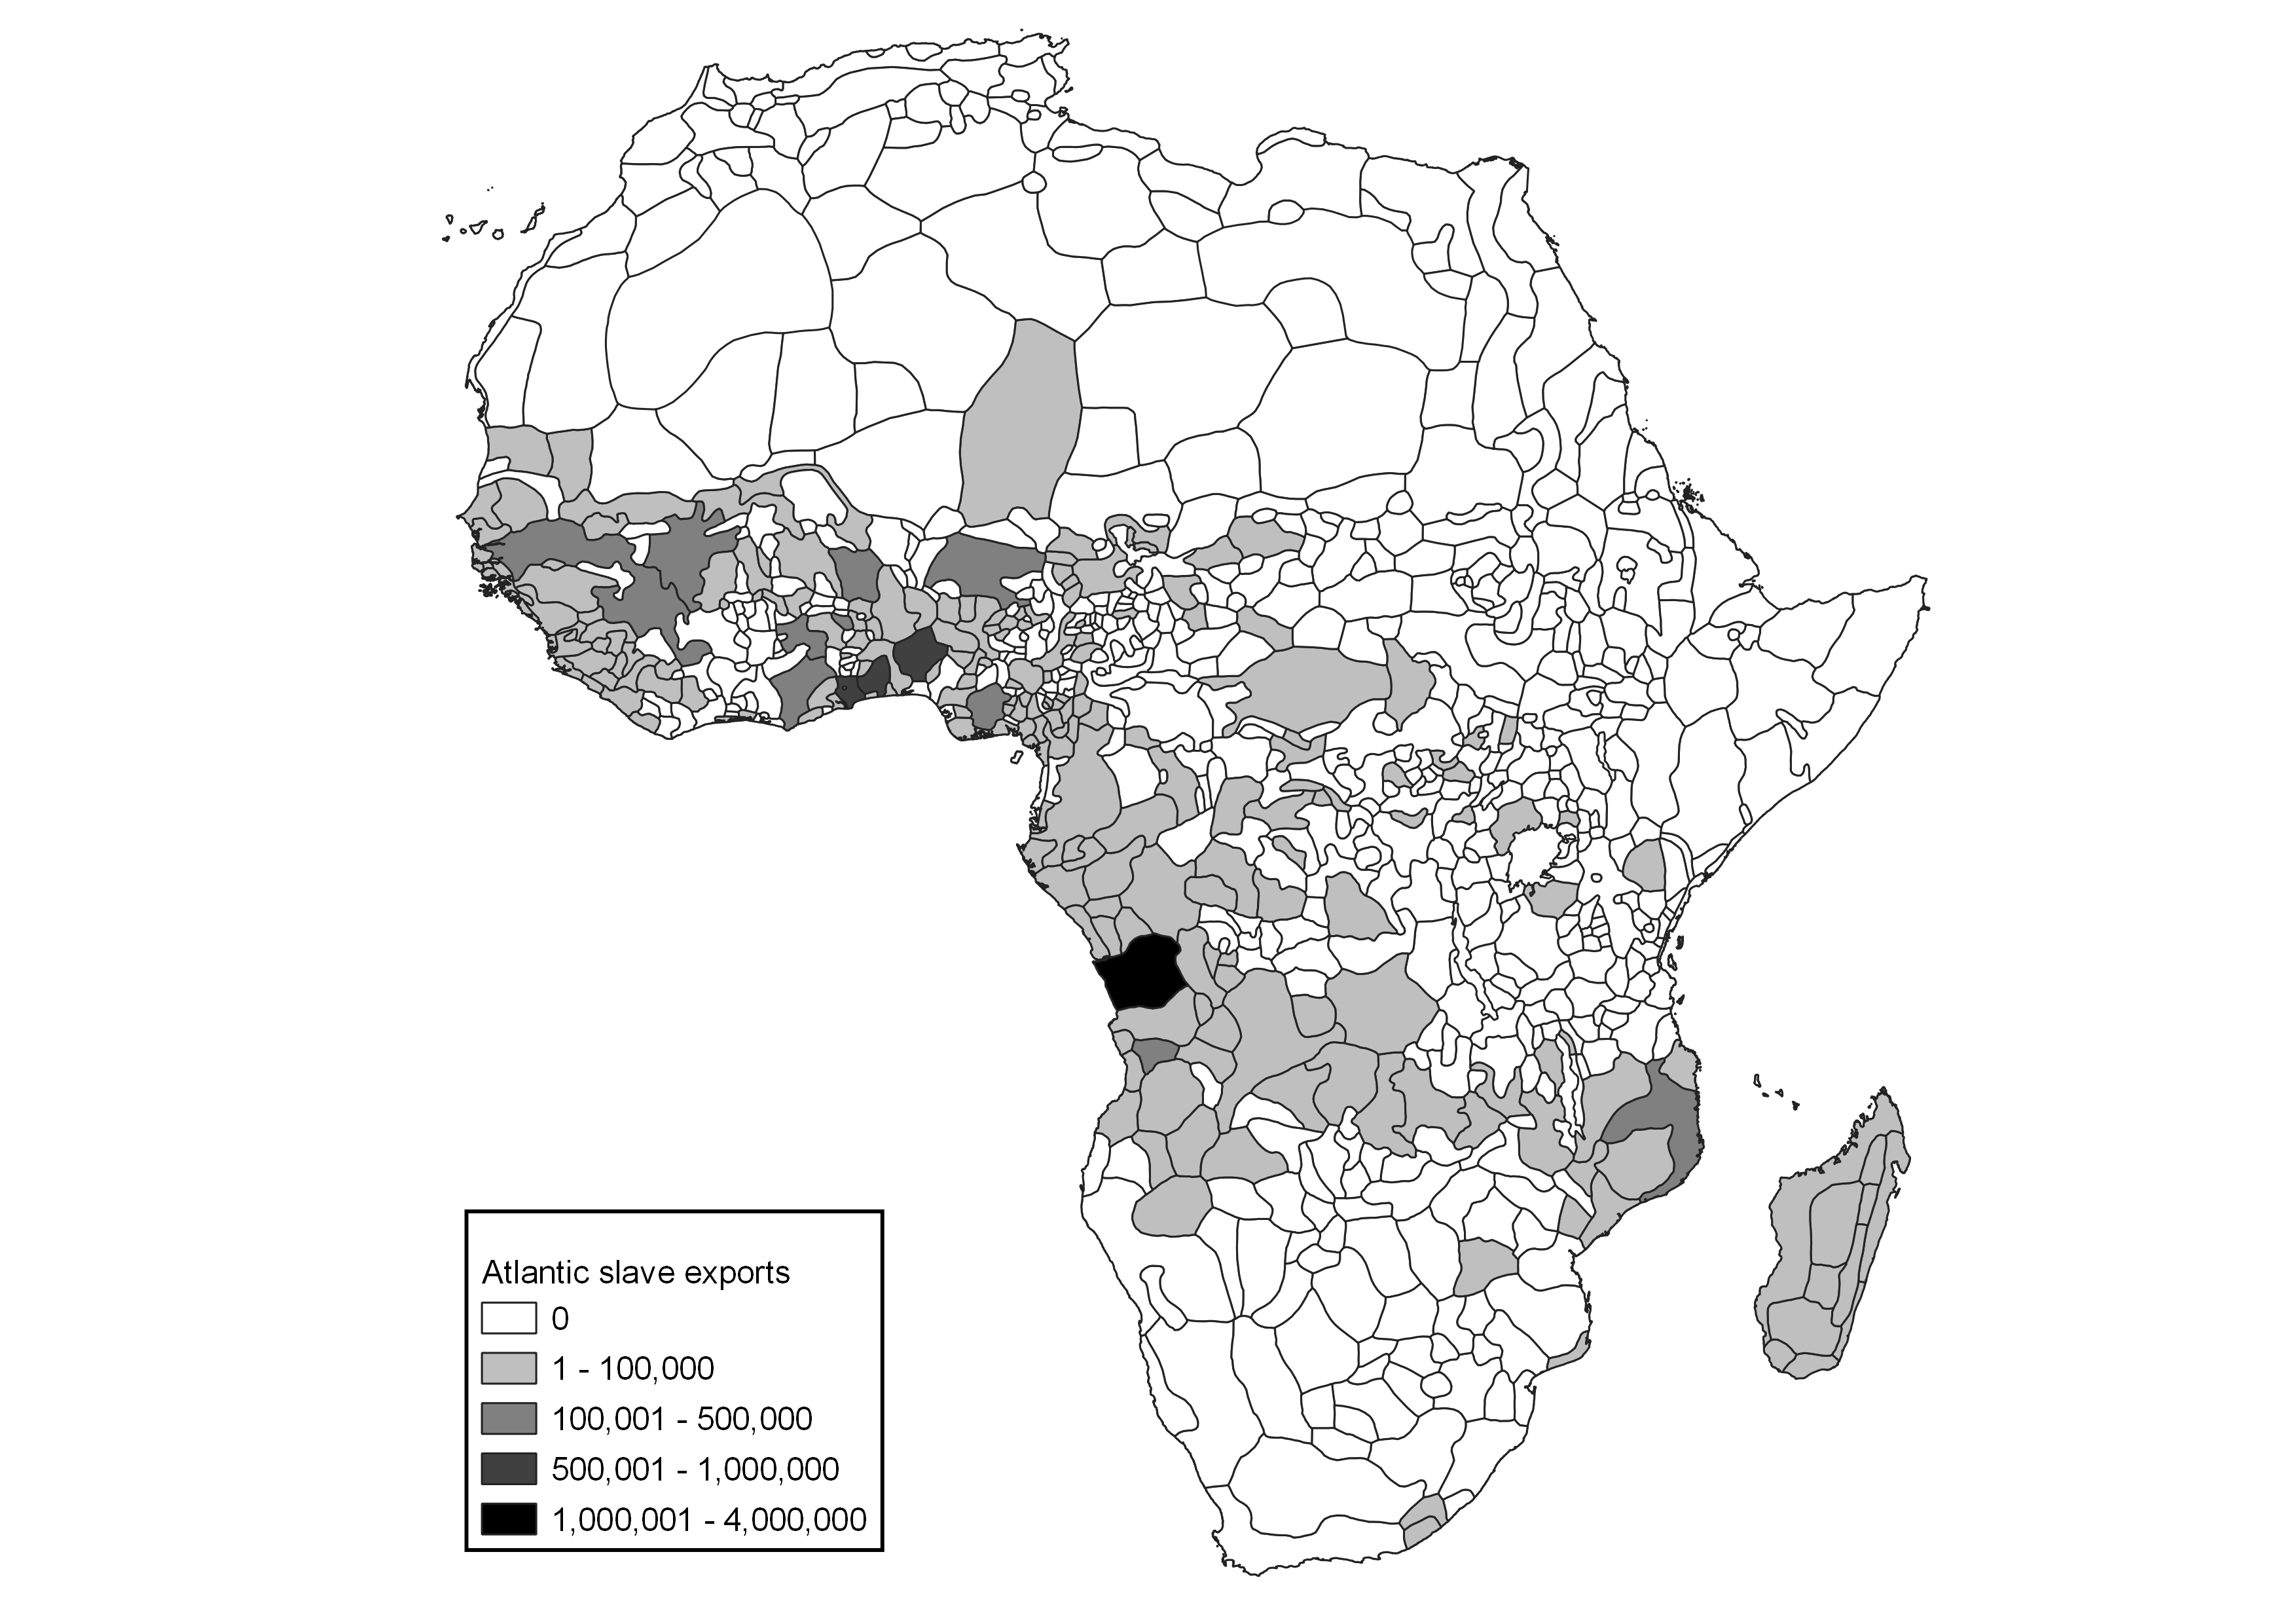
\includegraphics[scale = 0.45]{Final/Figure 1 - Panel A.png}
\label{}
\centering

Source: Own elaboration based on data sets of Nunn, N., \& Wantchekon, L. (2011): The slave trade and the origins of mistrust in Africa. American Economic Review.
\end{figure}

\begin{figure}[H]
\caption{Panel B. Indian slave exports}
\centering
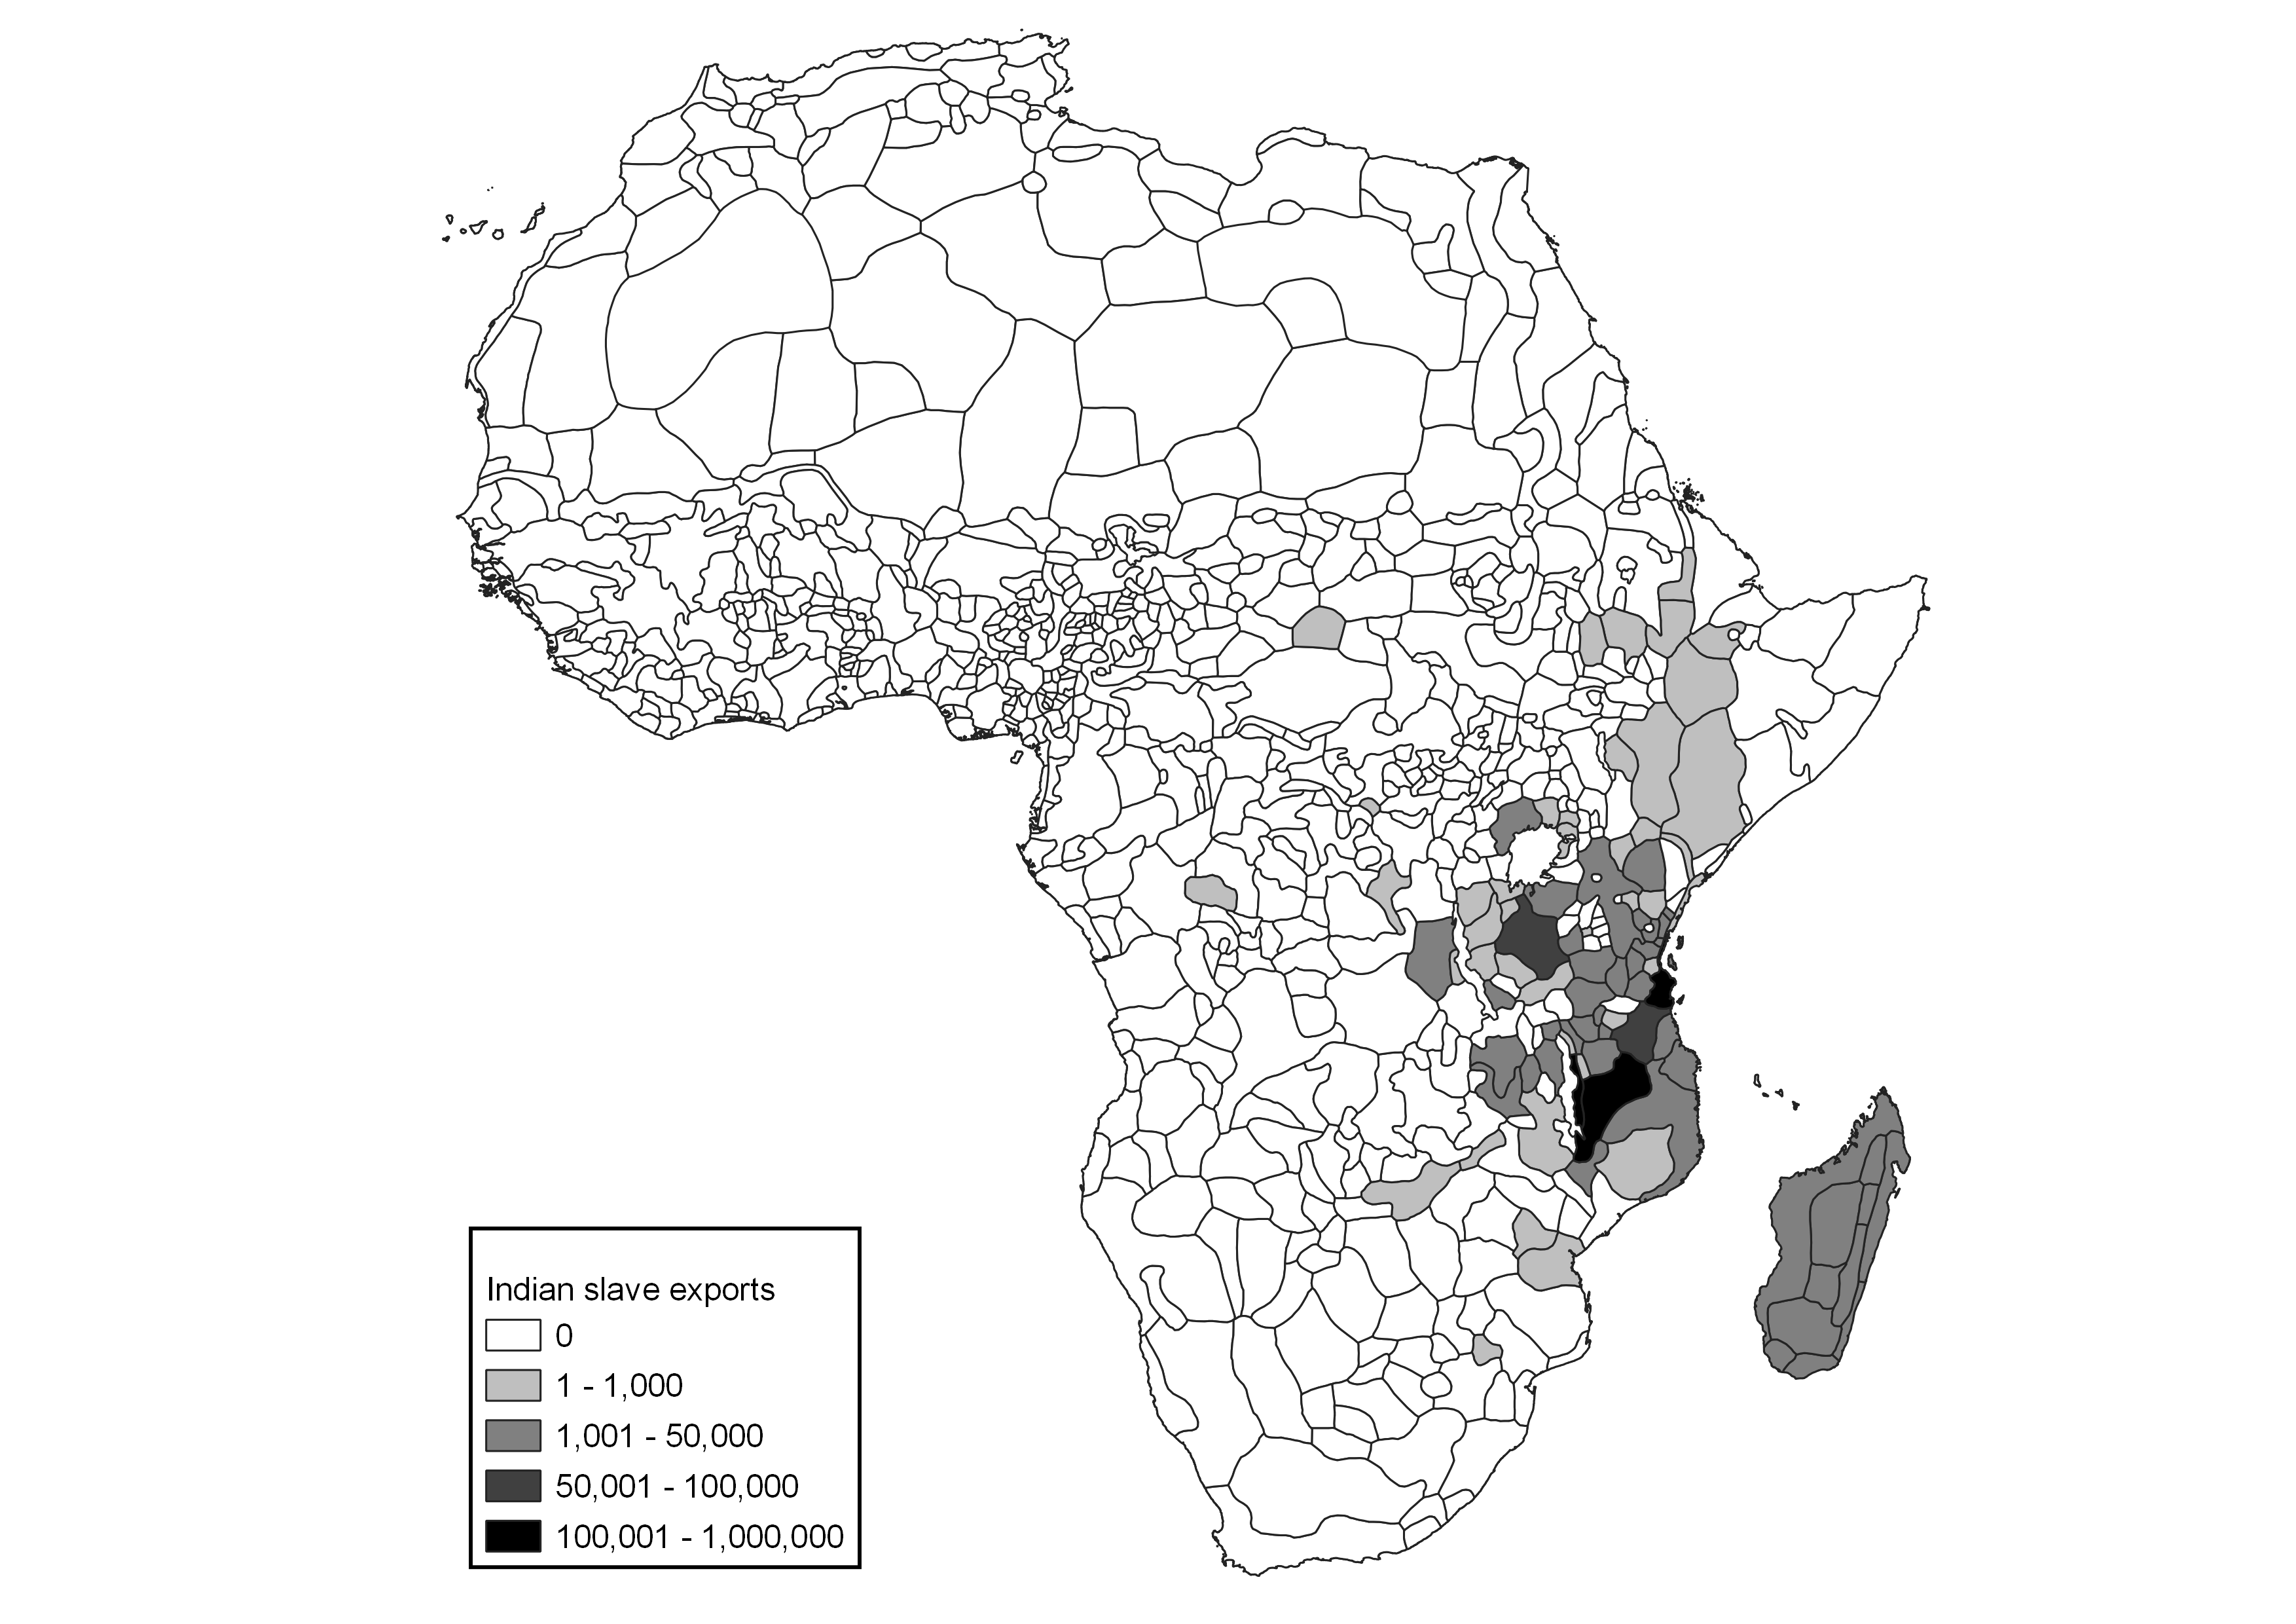
\includegraphics[scale = 0.45]{Final/Figure 1 - Panel B.png}
\label{}
\centering

Source: Own elaboration based on data sets of Nunn, N., \& Wantchekon, L. (2011): The slave trade and the origins of mistrust in Africa. American Economic Review.
\end{figure}



\section*{\textcolor{officegreen}{New maps}}

From here we present a series of subsections with their corresponding maps that seek to present additional information to the original maps of the paper. These sections are: First, Atlantic slave exports and maps of exploration routes by time periods. Second, Indian slave exports and maps of exploration routes by time periods. Finally, the total number of slaves exported by period of time.


\section*{\textcolor{officegreen}{Atlantic slave exports and explorer routes maps by periods of time}}

Here is a series of maps that show the export of slaves to the Atlantic in the periods 1400-1599, 1600-1699, 1700-1799 and 1800-1899, correspondingly. In turn, for each period, the explorer routes are shown in blue. It can be seen how over the years the number of routes increased and they have terminals in the different ports used for the export of slaves.

\begin{figure}[H]
\caption{Atlantic slave exports and explorer routes in the period 1400 -1599}
\centering
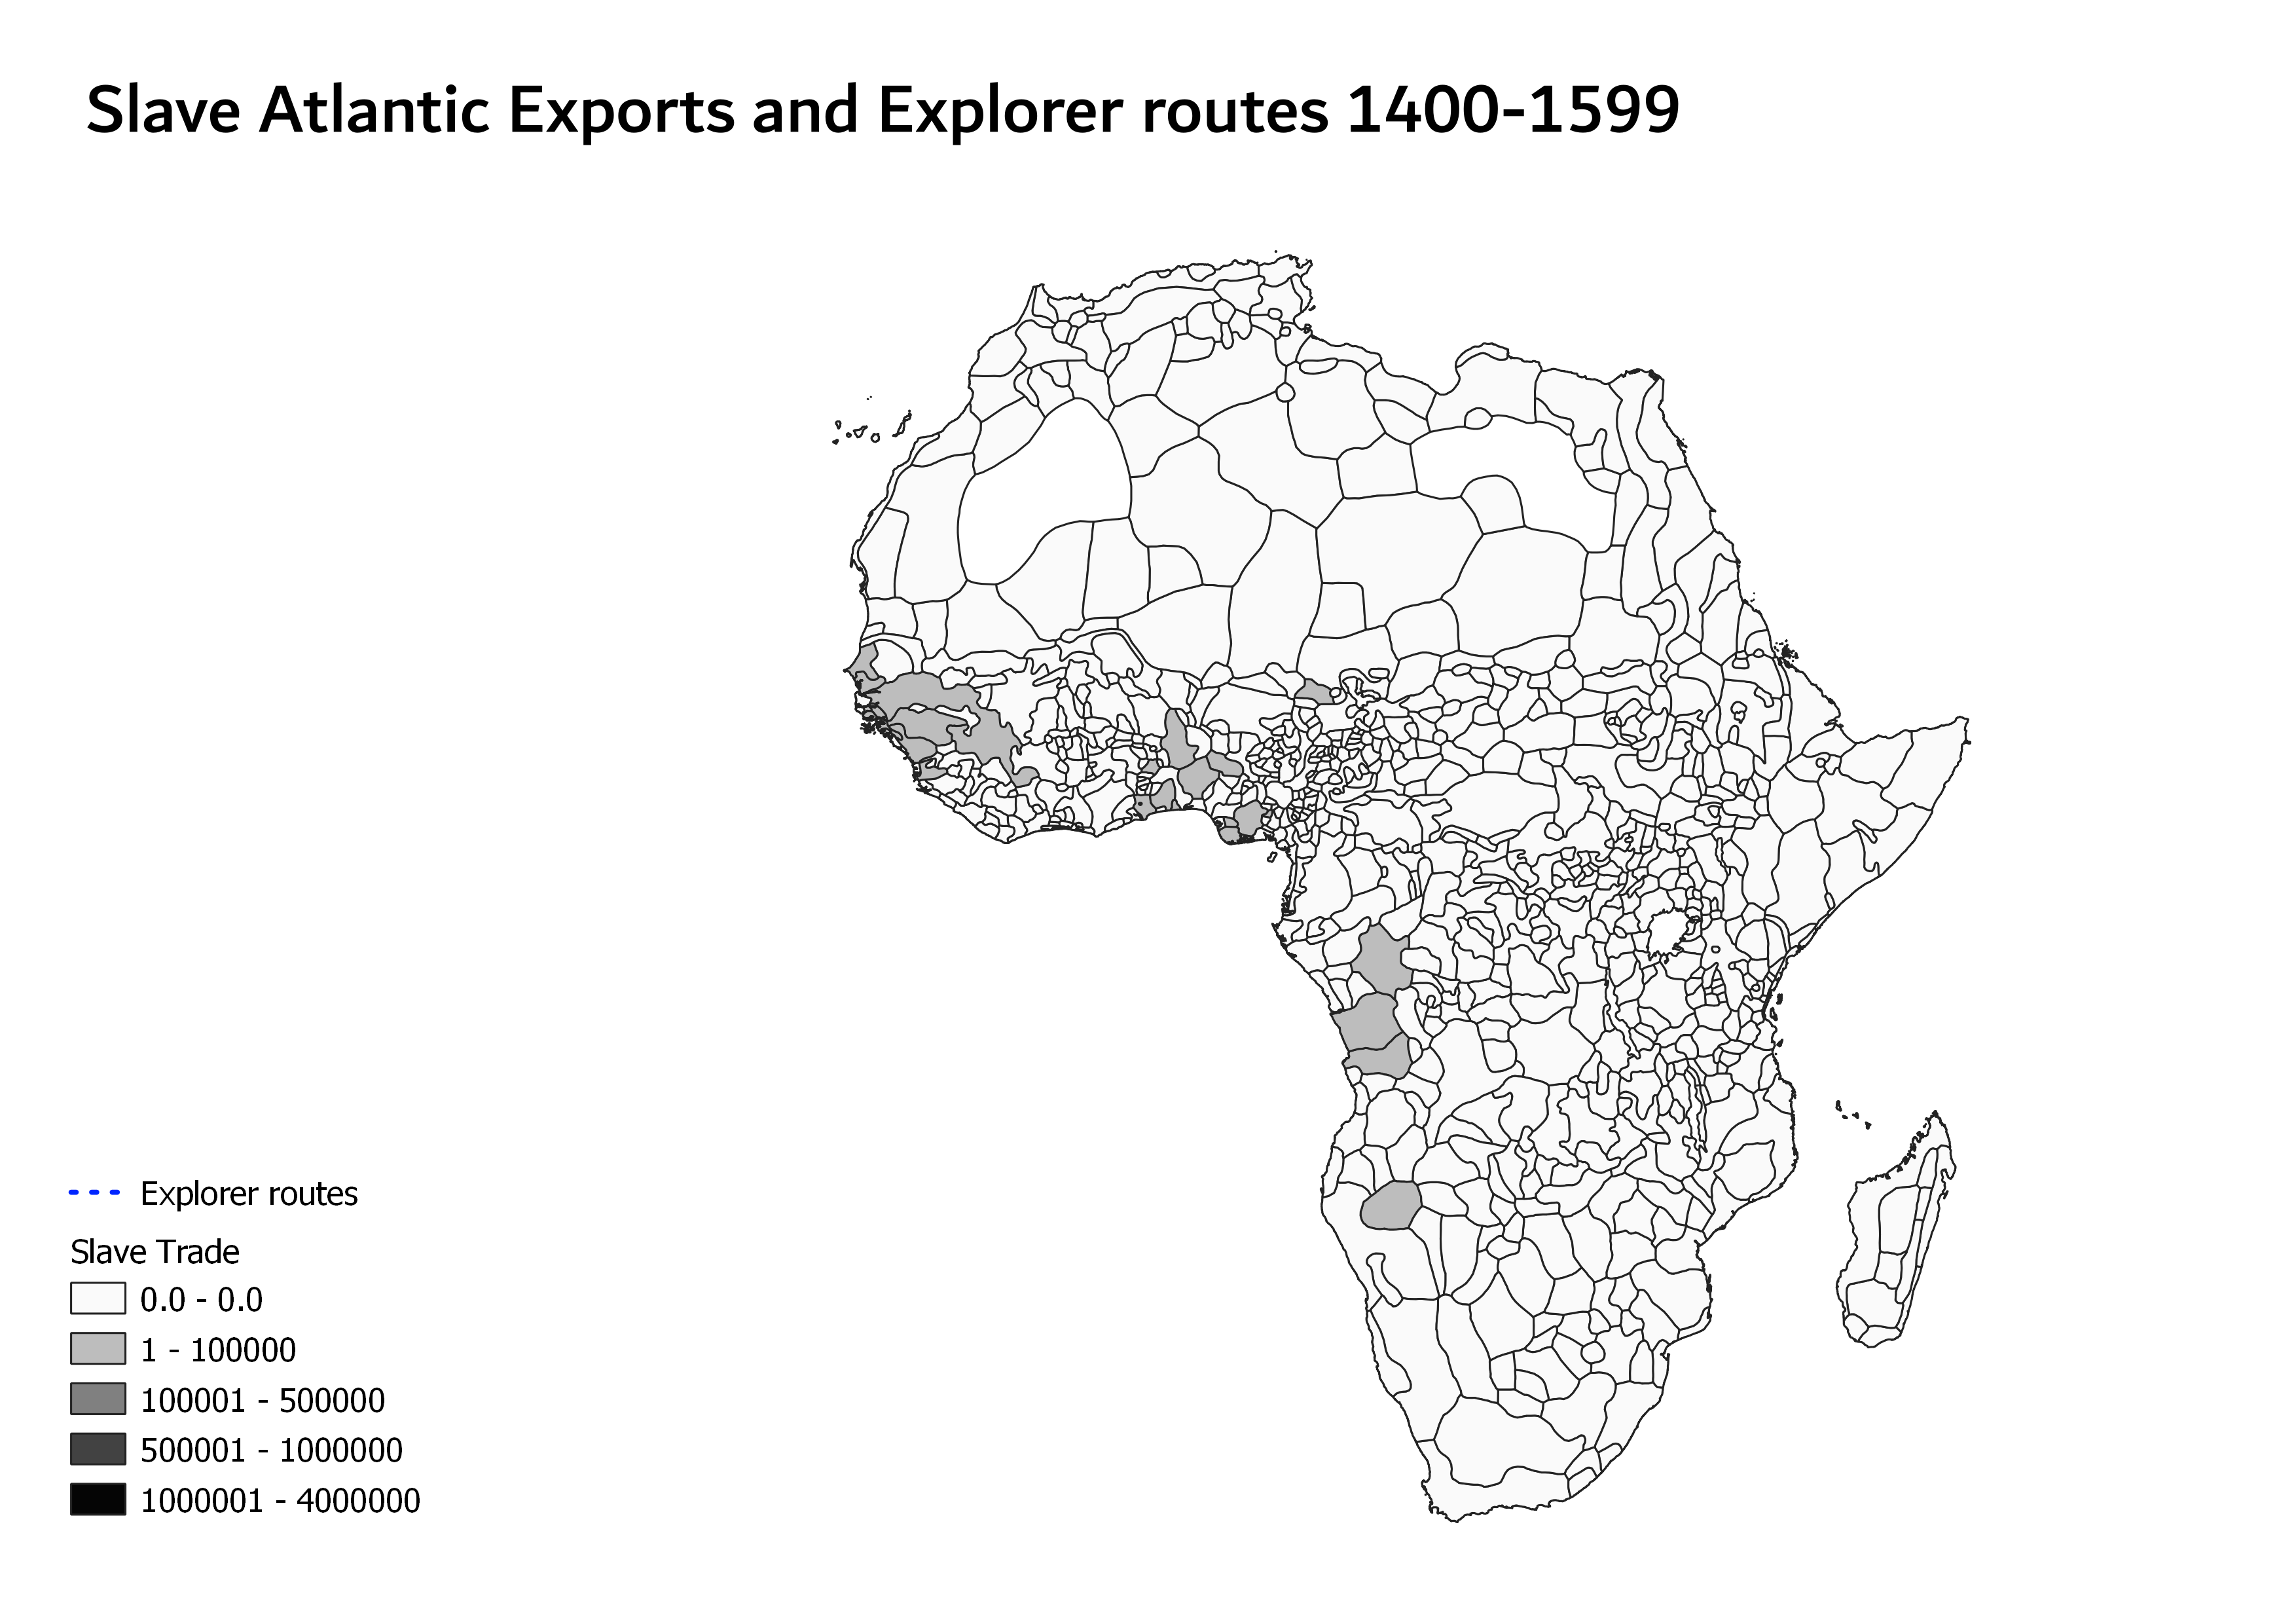
\includegraphics[scale = 0.45]{Final/Slave atlantic exports and explorer routes 1400 -1599.png}
\label{}
\centering

Source: Own elaboration based on data sets of Nunn, N., \& Wantchekon, L. (2011): The slave trade and the origins of mistrust in Africa. American Economic Review.
\end{figure}

\begin{figure}[H]
\caption{Atlantic slave exports and explorer routes in the period 1600 -1699}
\centering
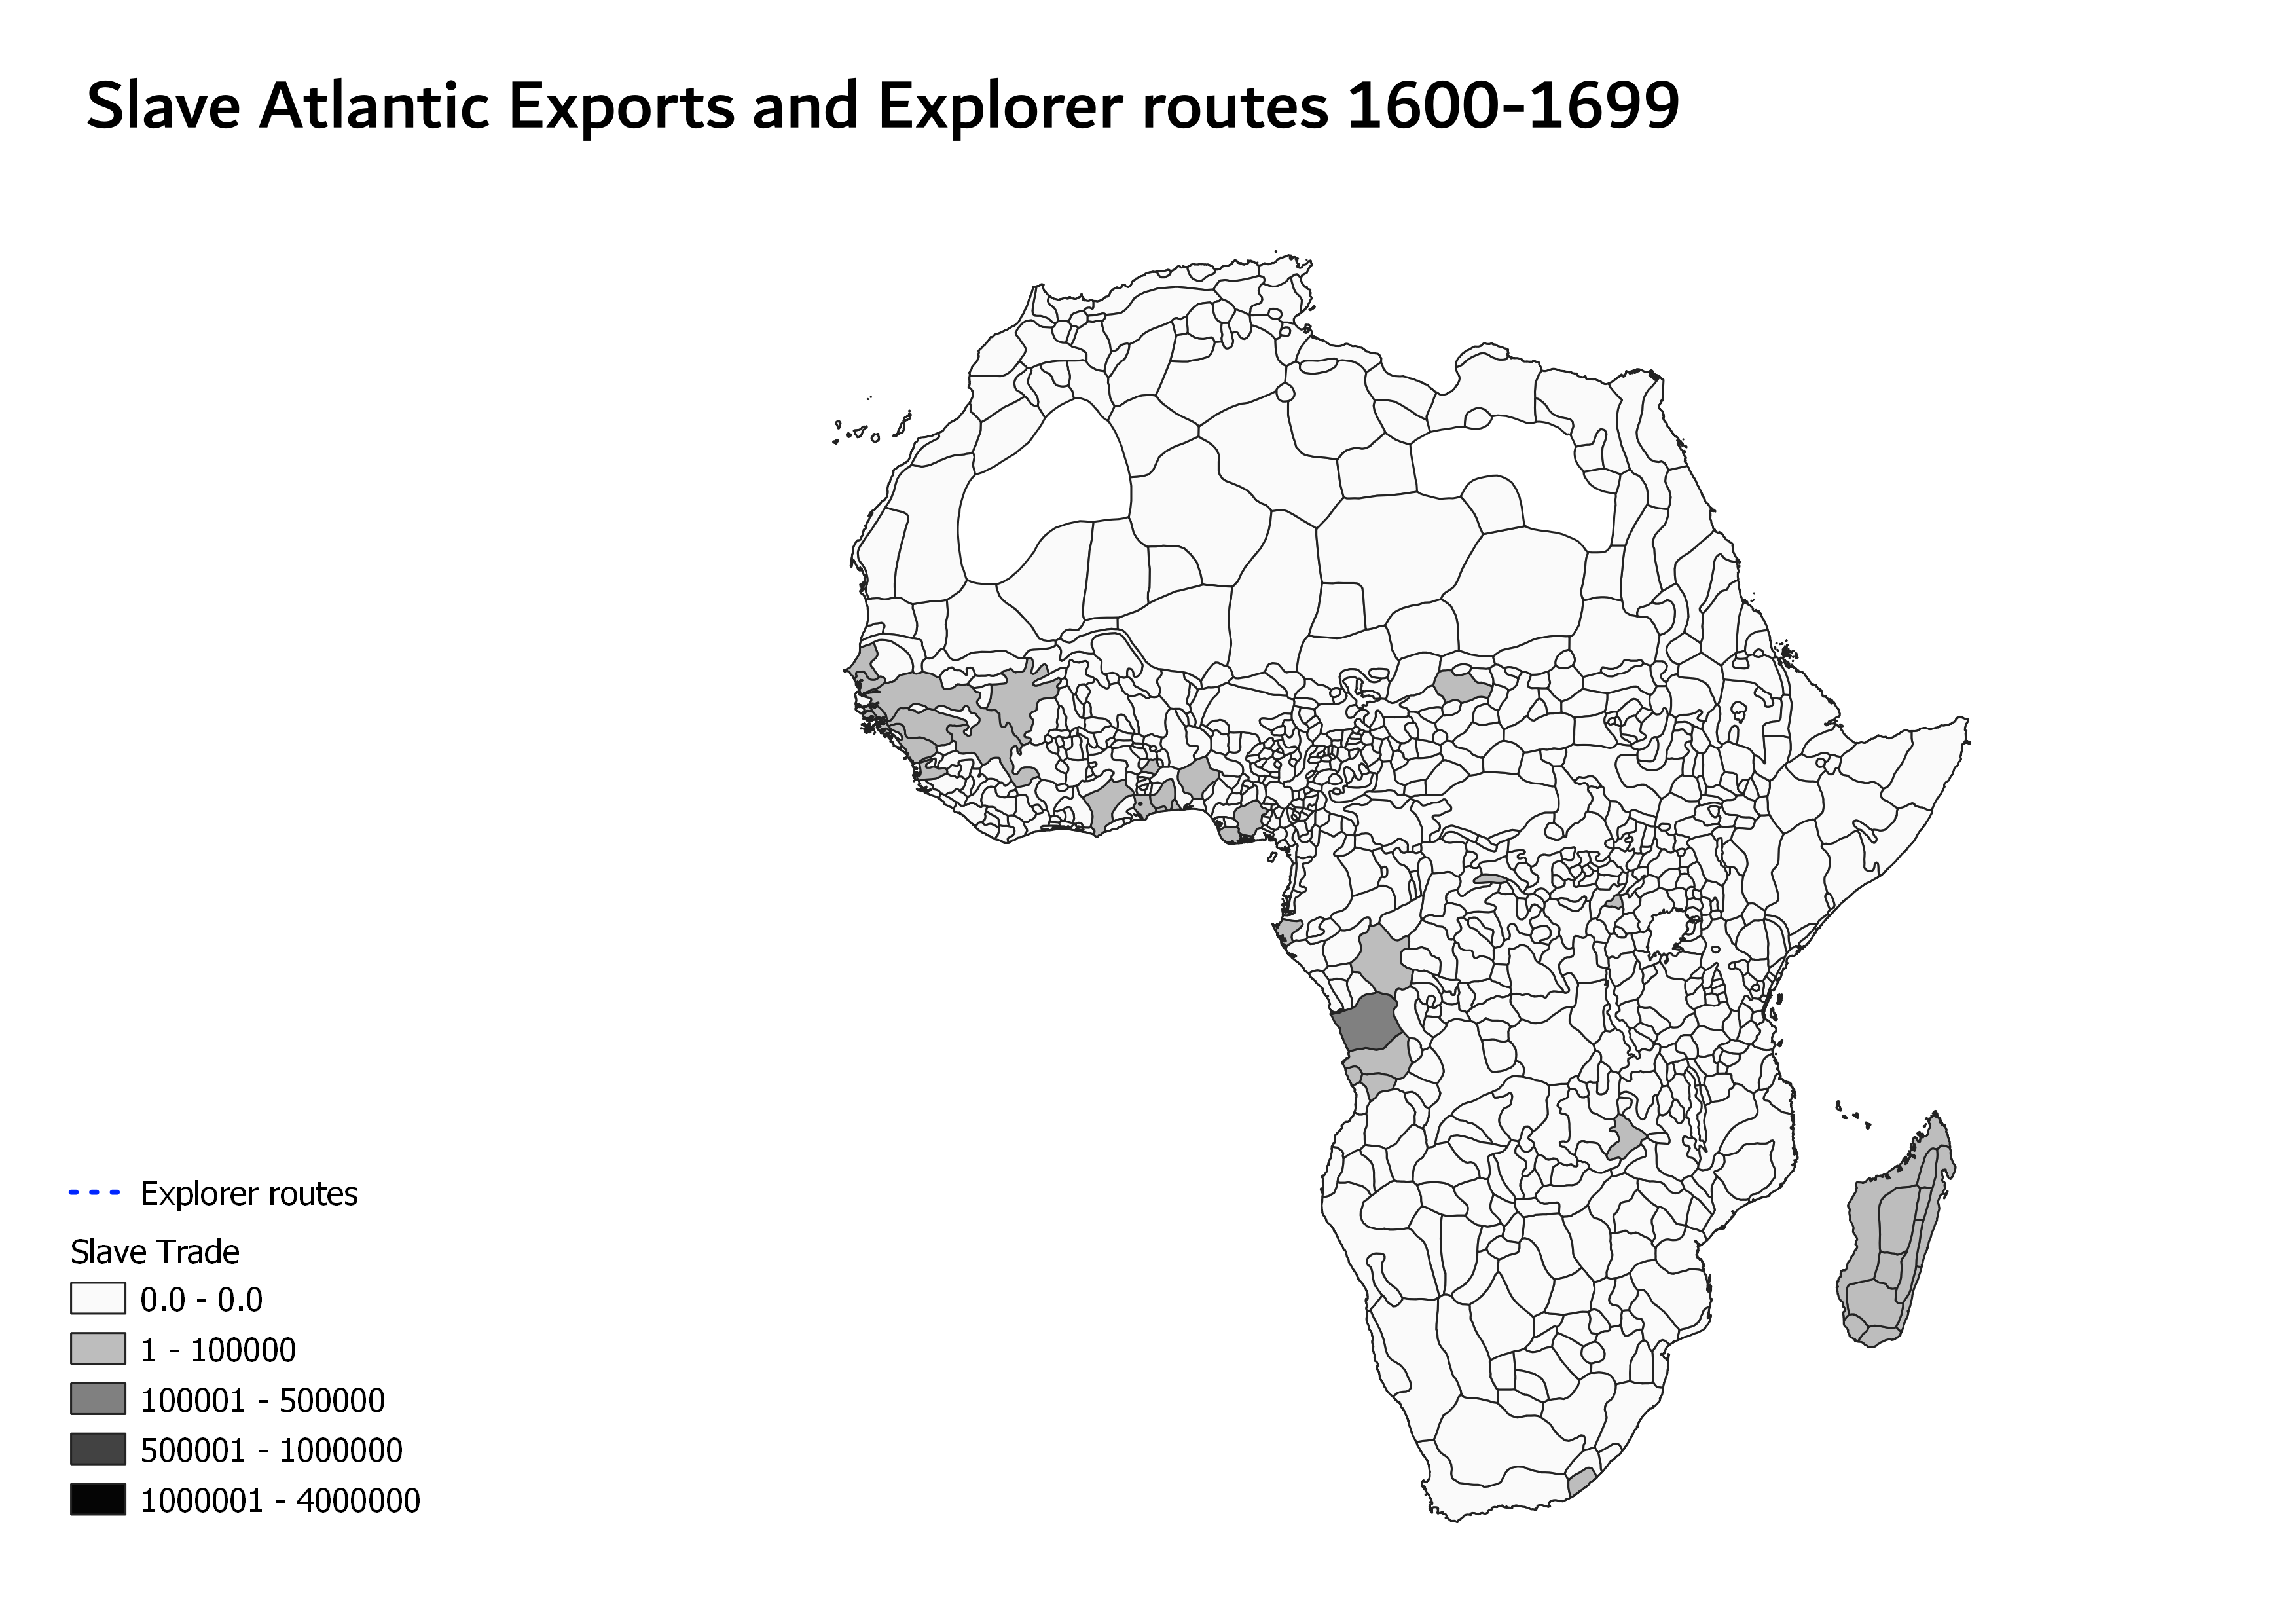
\includegraphics[scale = 0.45]{Final/Slave atlantic exports and explorer routes 1600-1699.png}
\label{}
\centering

Source: Own elaboration based on data sets of Nunn, N., \& Wantchekon, L. (2011): The slave trade and the origins of mistrust in Africa. American Economic Review.
\end{figure}


\begin{figure}[H]
\caption{Atlantic slave exports and explorer routes in the period 1700 -1799}
\centering
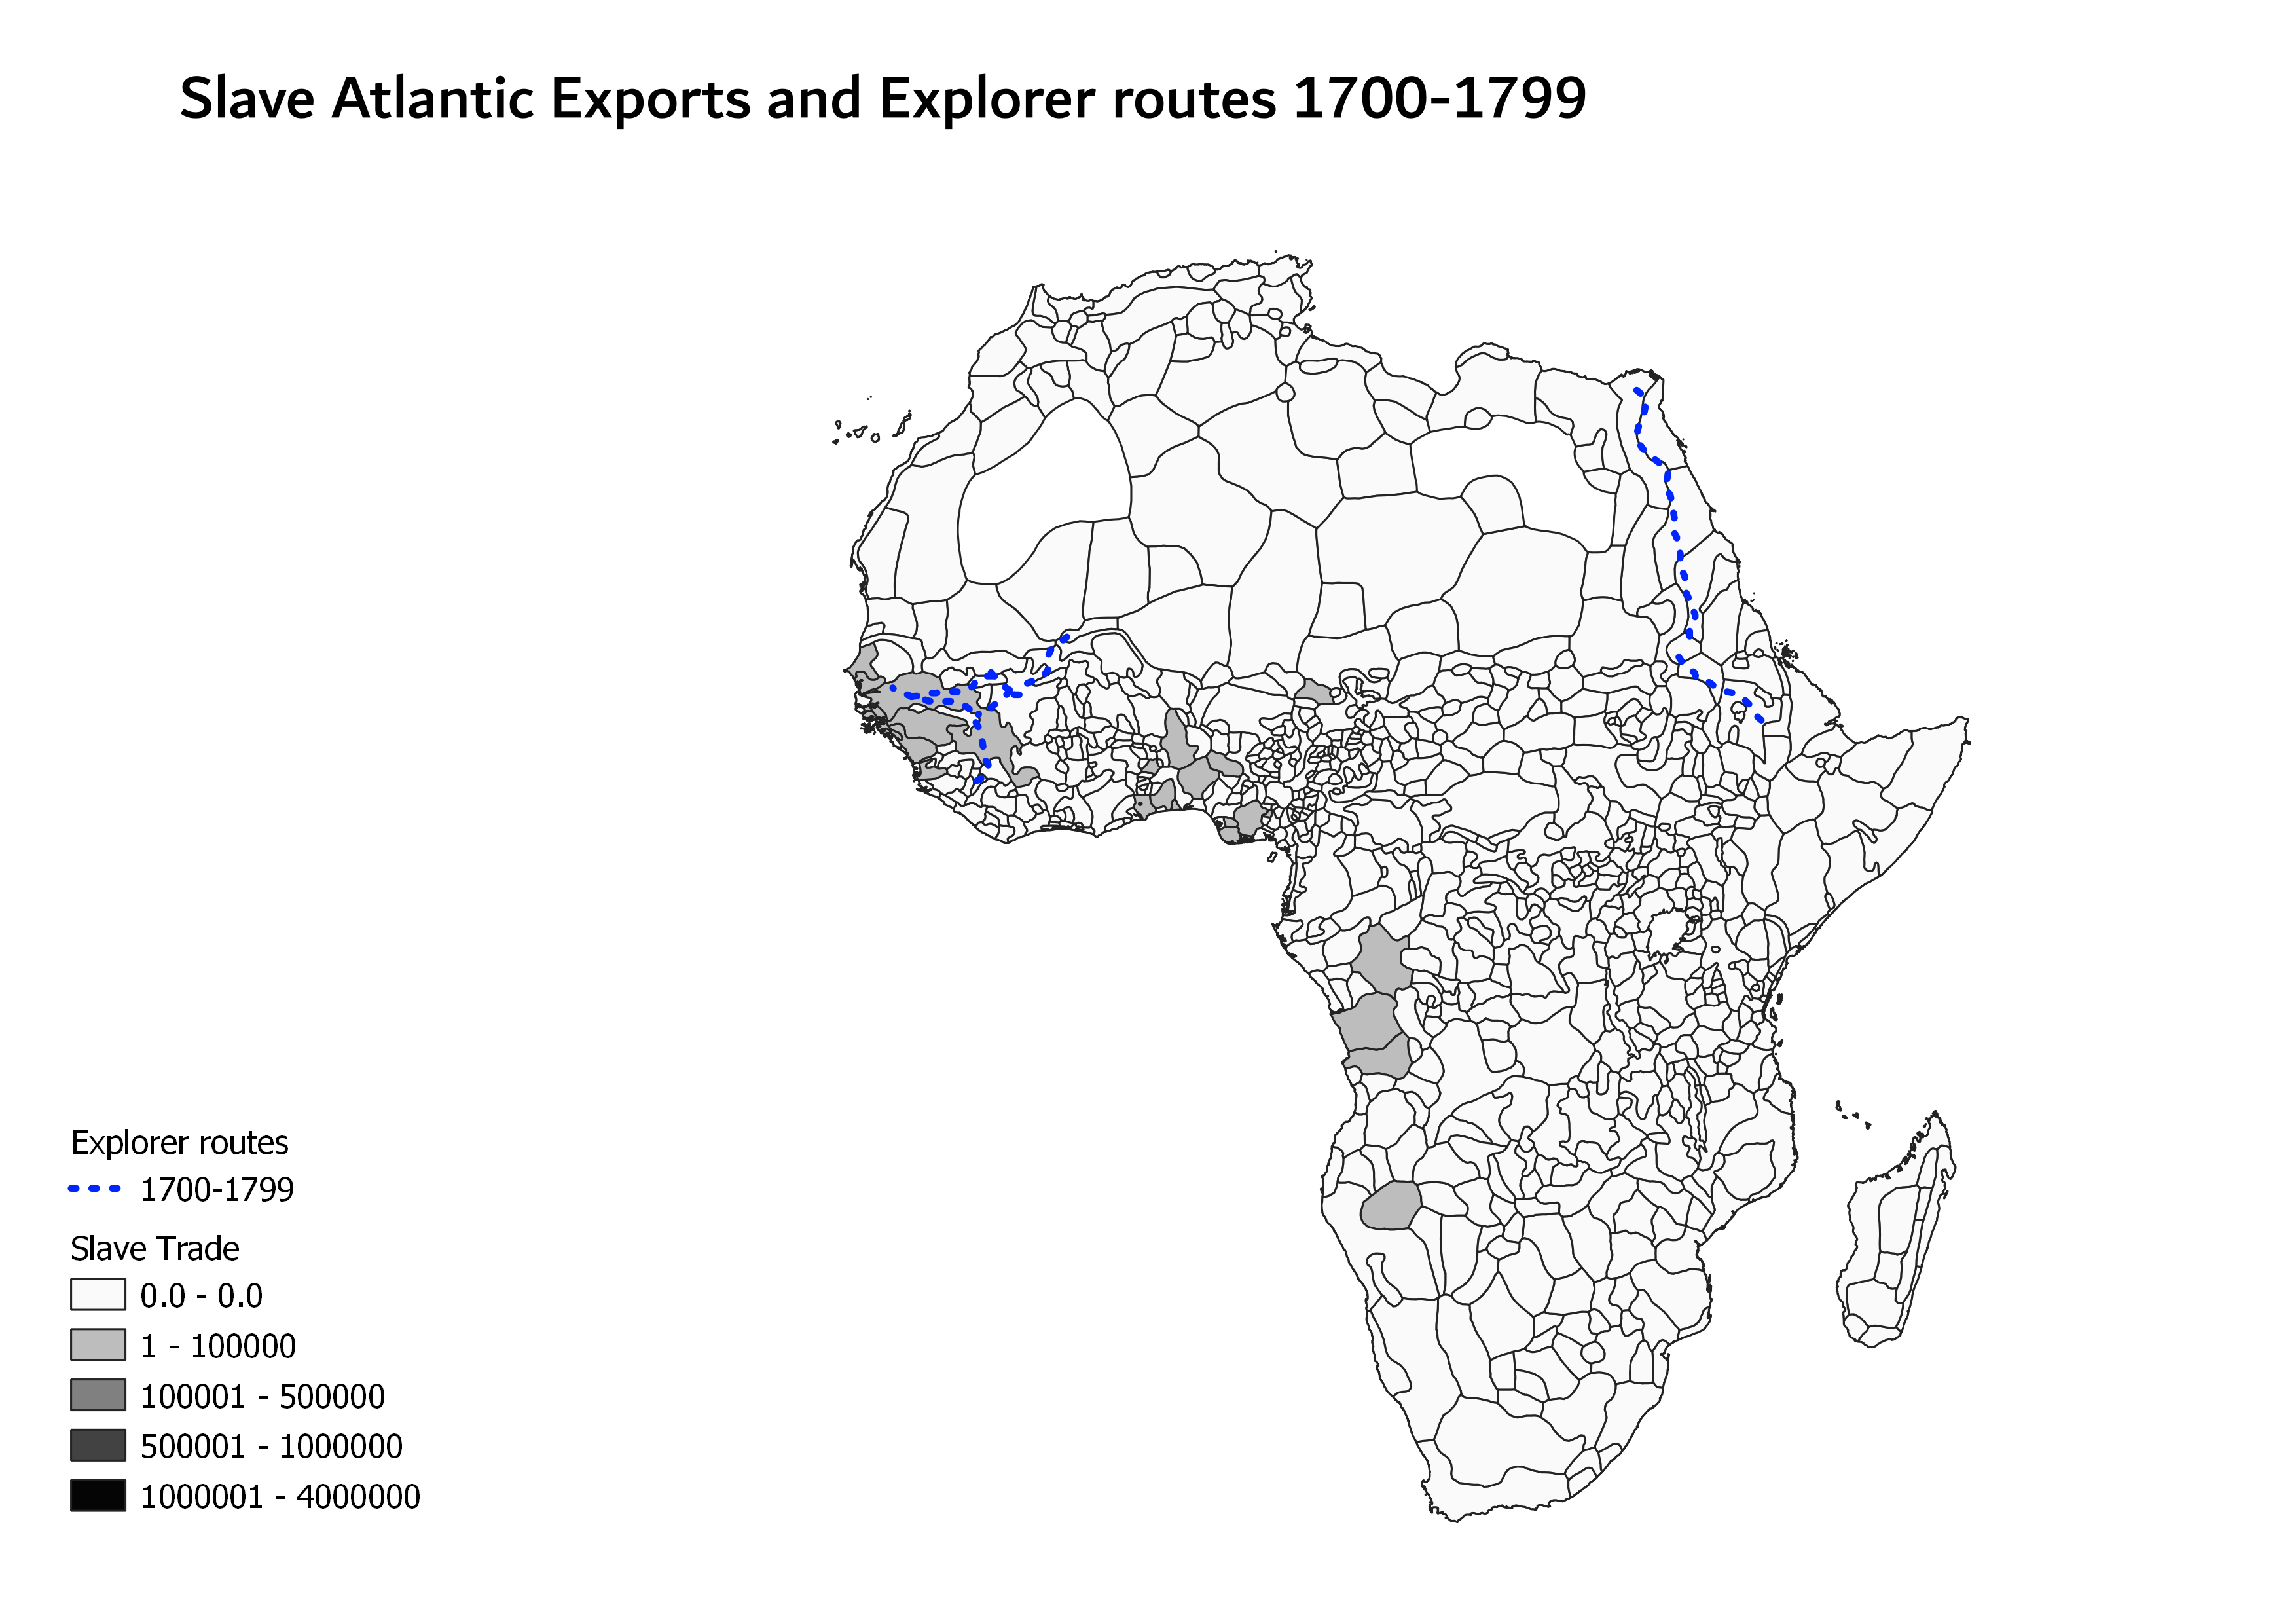
\includegraphics[scale = 0.45]{Final/Slave atlantic exports and explorer routes 1700 - 1799.png}
\label{}
\centering

Source: Own elaboration based on data sets of Nunn, N., \& Wantchekon, L. (2011): The slave trade and the origins of mistrust in Africa. American Economic Review.
\end{figure}


\begin{figure}[H]
\caption{Atlantic slave exports and explorer routes in the period 1800 -1899}
\centering
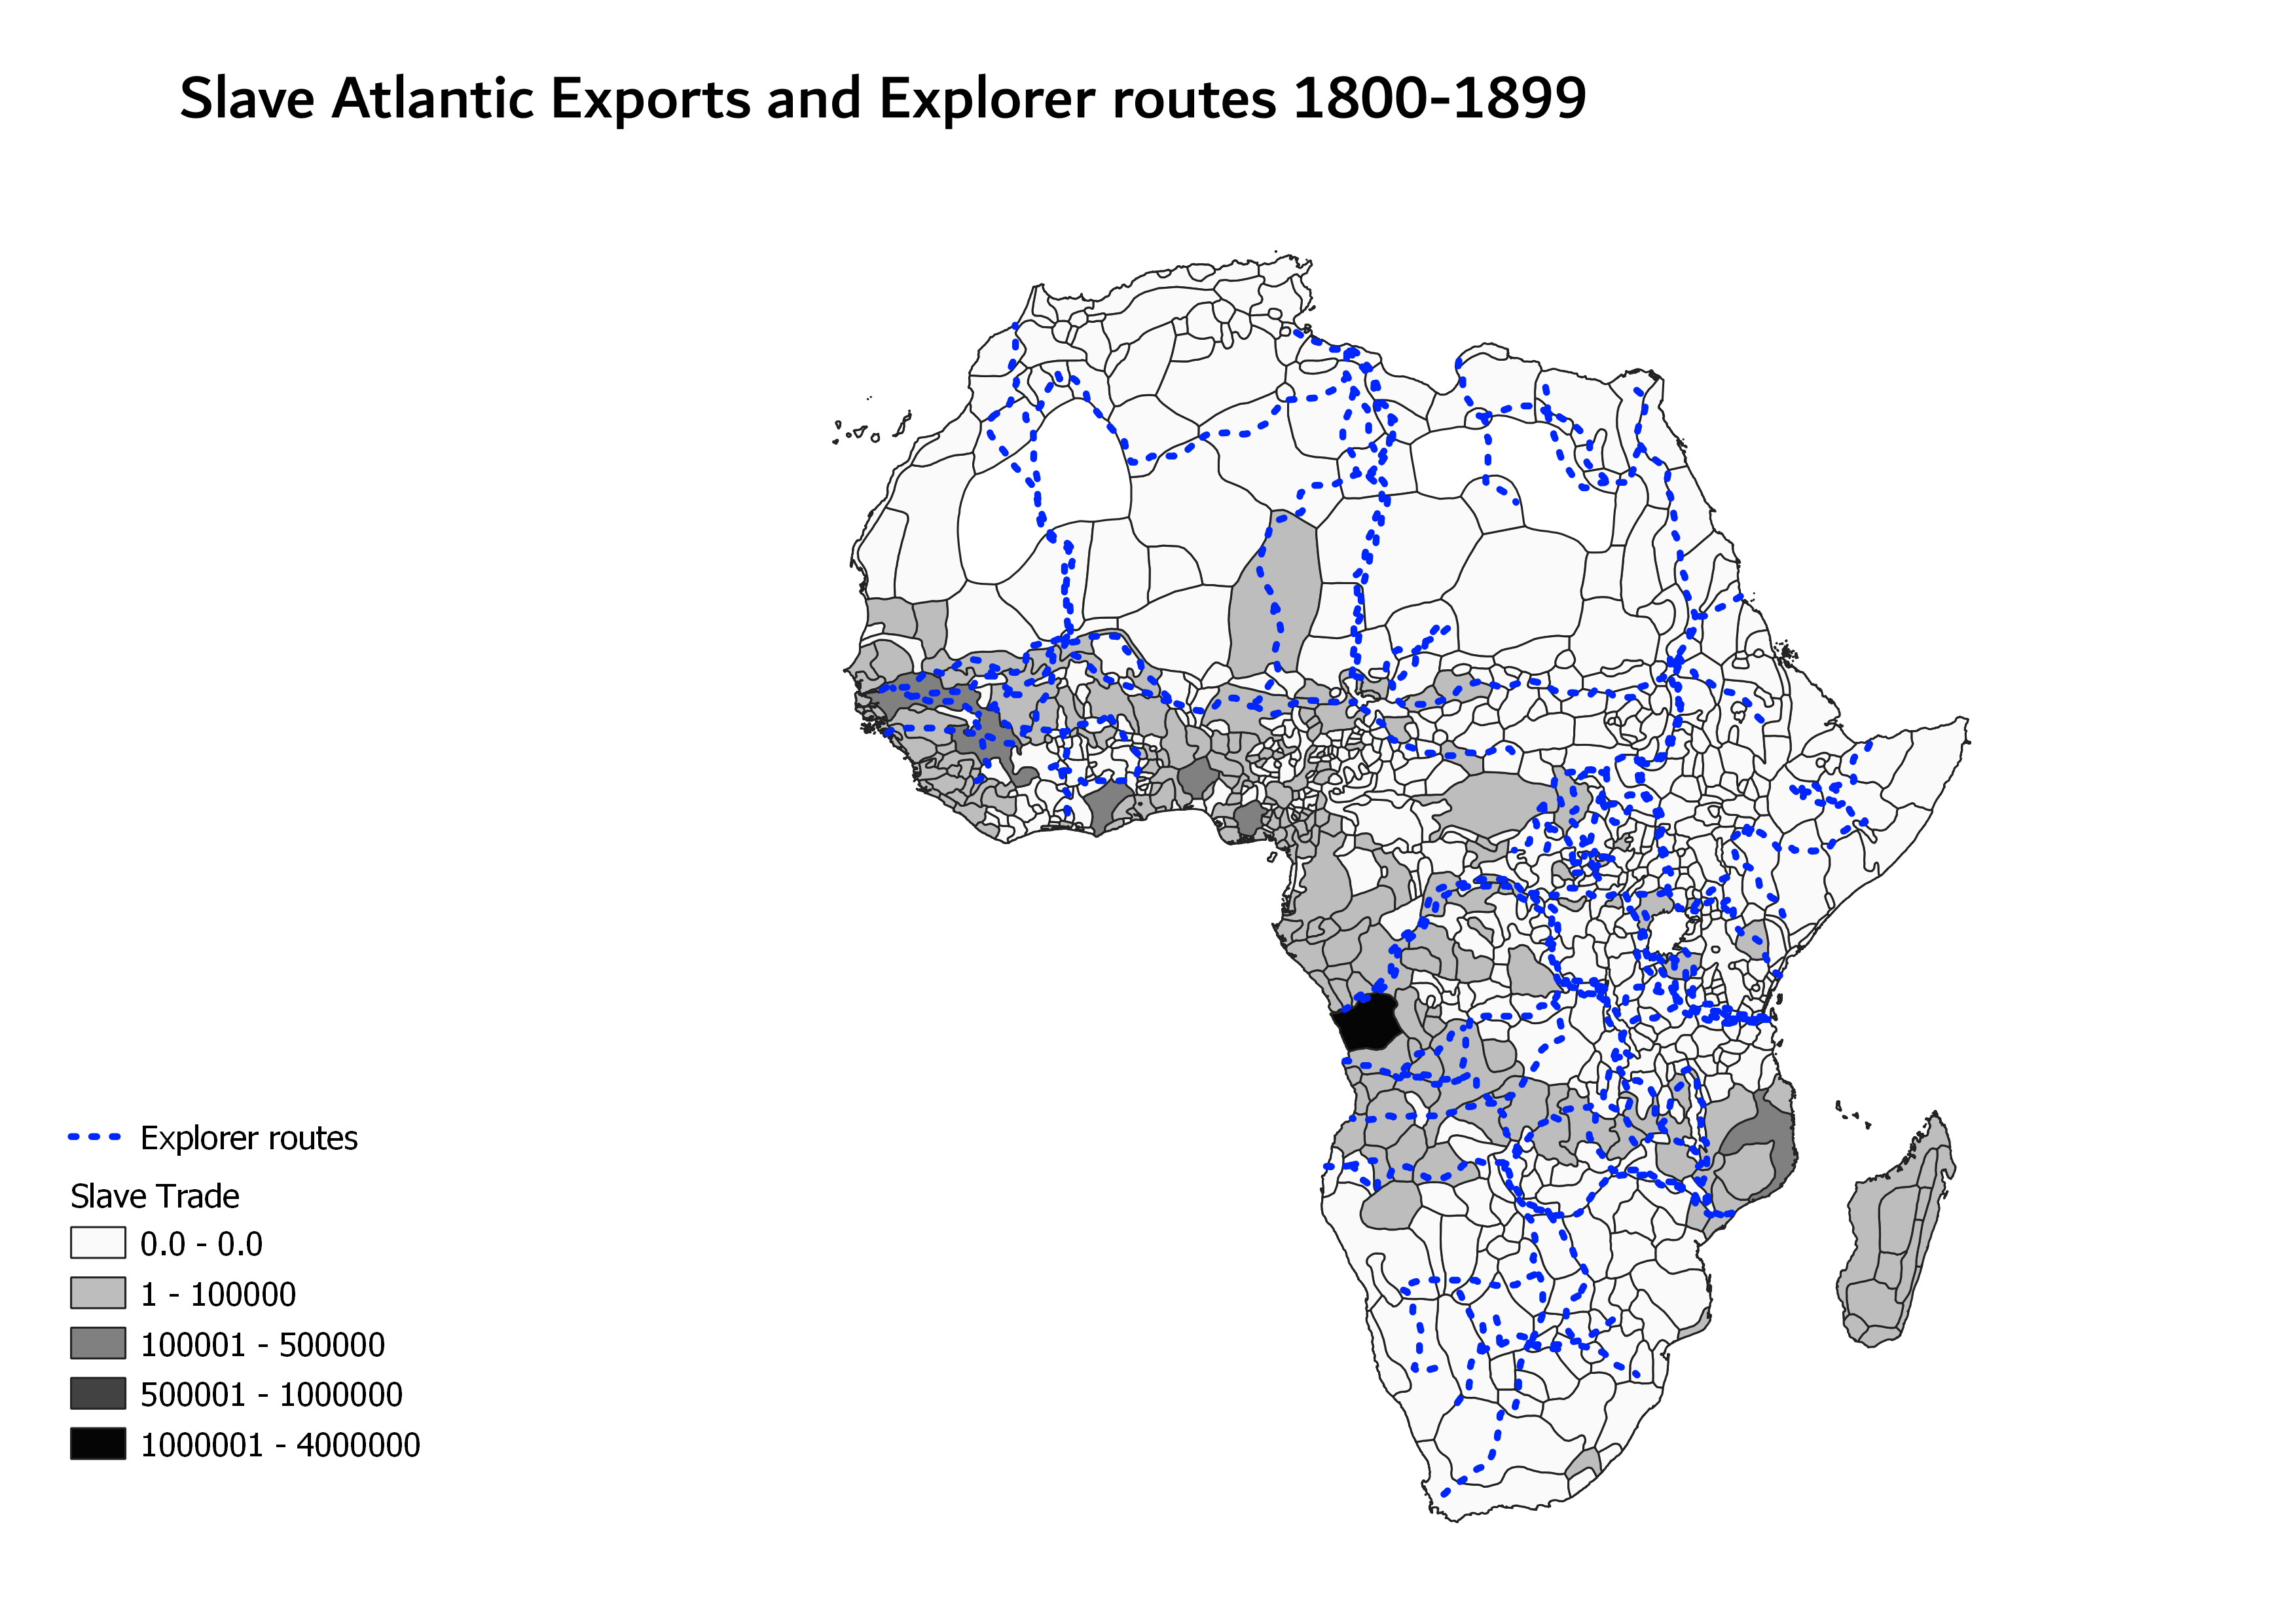
\includegraphics[scale = 0.45]{Final/Slave atlantic exports and explorer routes 1800-1899.png}
\label{}
\centering

Source: Own elaboration based on data sets of Nunn, N., \& Wantchekon, L. (2011): The slave trade and the origins of mistrust in Africa. American Economic Review.
\end{figure}



\section*{\textcolor{officegreen}{Atlantic slave exports and explorer routes maps by periods of time}}

Here we show a map that responds to an exploratory exercise of crossing two datasets used by Nunn, N., firstly, the scales of slave exports to the Atlantic along with the routes of explorers. The additional element is to use the shapefile generated by Nunn, N. (2010) in the paper: "Religious conversion in colonial Africa". In this way, the different locations of the Catholic and Protestant mission stations, respectively, can be verified with yellow, aqua green and red dots.

\begin{figure}[H]
\caption{Slave trade, missions and explorer routes}
\centering
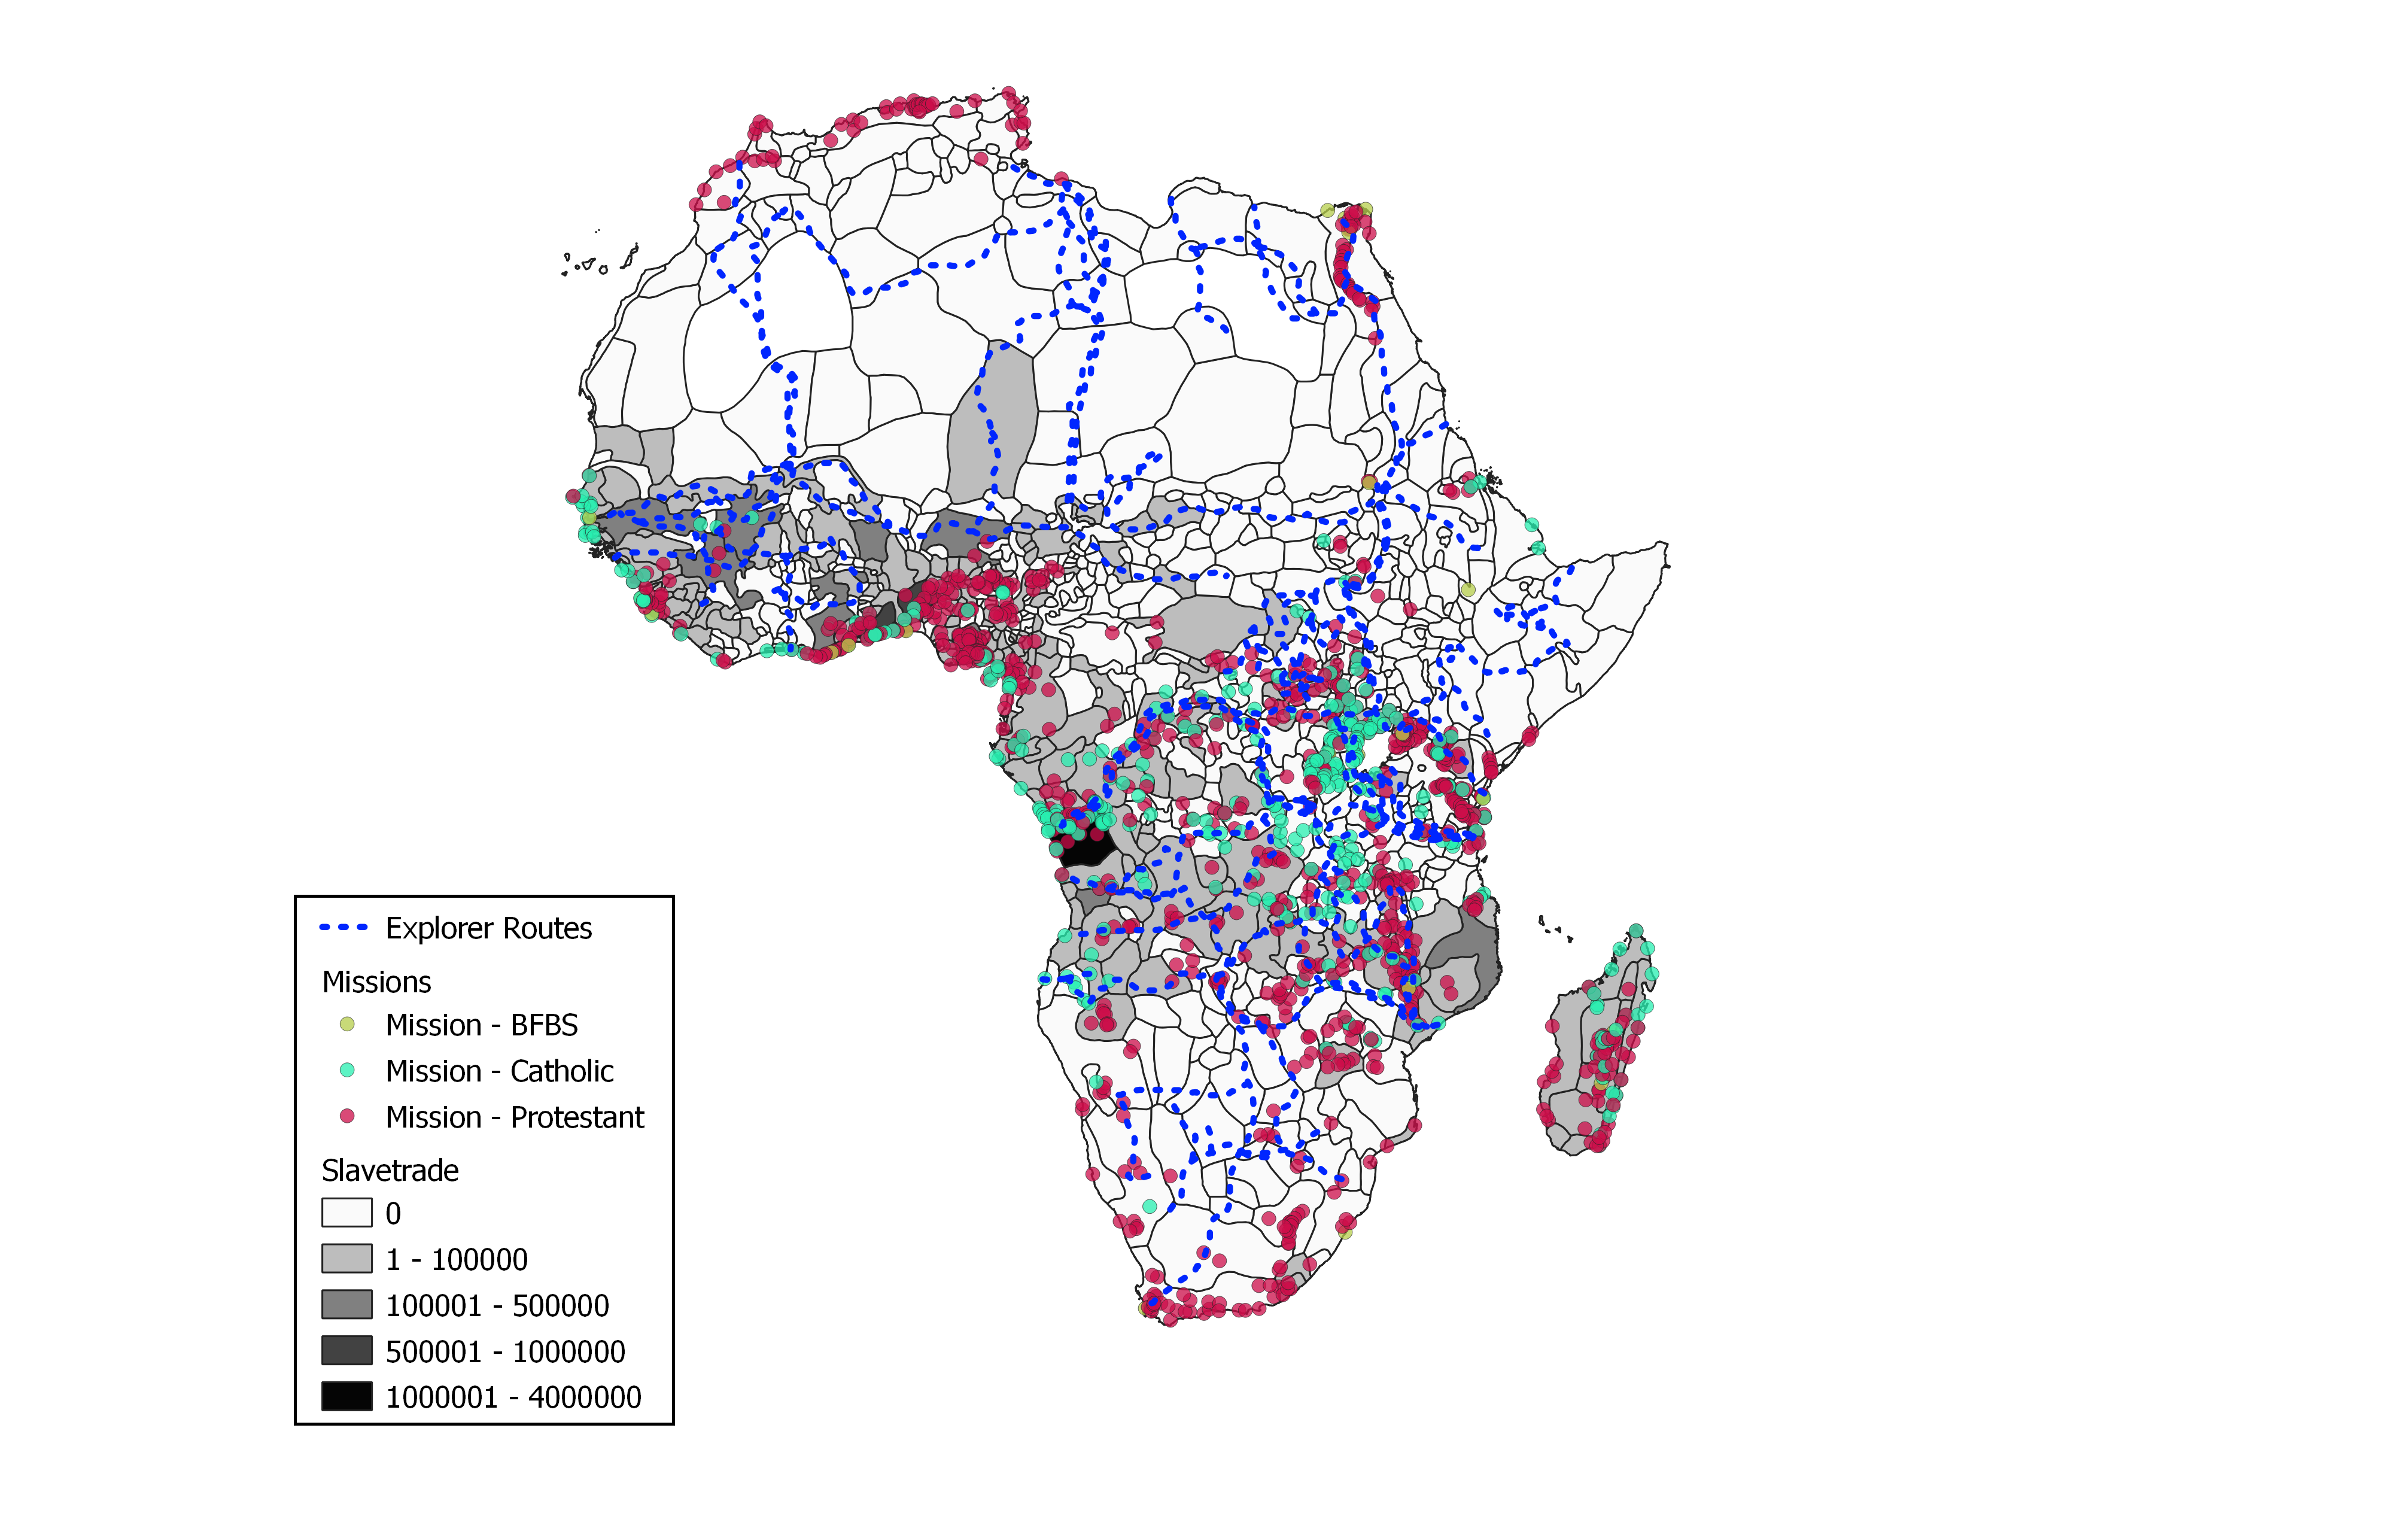
\includegraphics[scale = 0.45]{Final/Slave trade, missions and explorer final.png}
\label{}
\centering

Source: Own elaboration based on data sets of Nunn, N., \& Wantchekon, L. (2011): The slave trade and the origins of mistrust in Africa. American Economic Review and Nunn, N. (2010): Religious conversion in colonial Africa. American Economic Review.
\end{figure}

\section*{\textcolor{officegreen}{Total slave exports by periods of time}}

Here we show the total number of slaves exported from Africa, for a period of time from 1500 to 1800, using the same chromatic and quantile scale that Nunn, N., \& Wantchekon, L. (2011) follow. To do so, we form a new variable within the dataset presented by the authors to aggregate the number of slaves exported by destination and by time period.

\begin{figure}[H]
\caption{}
\centering
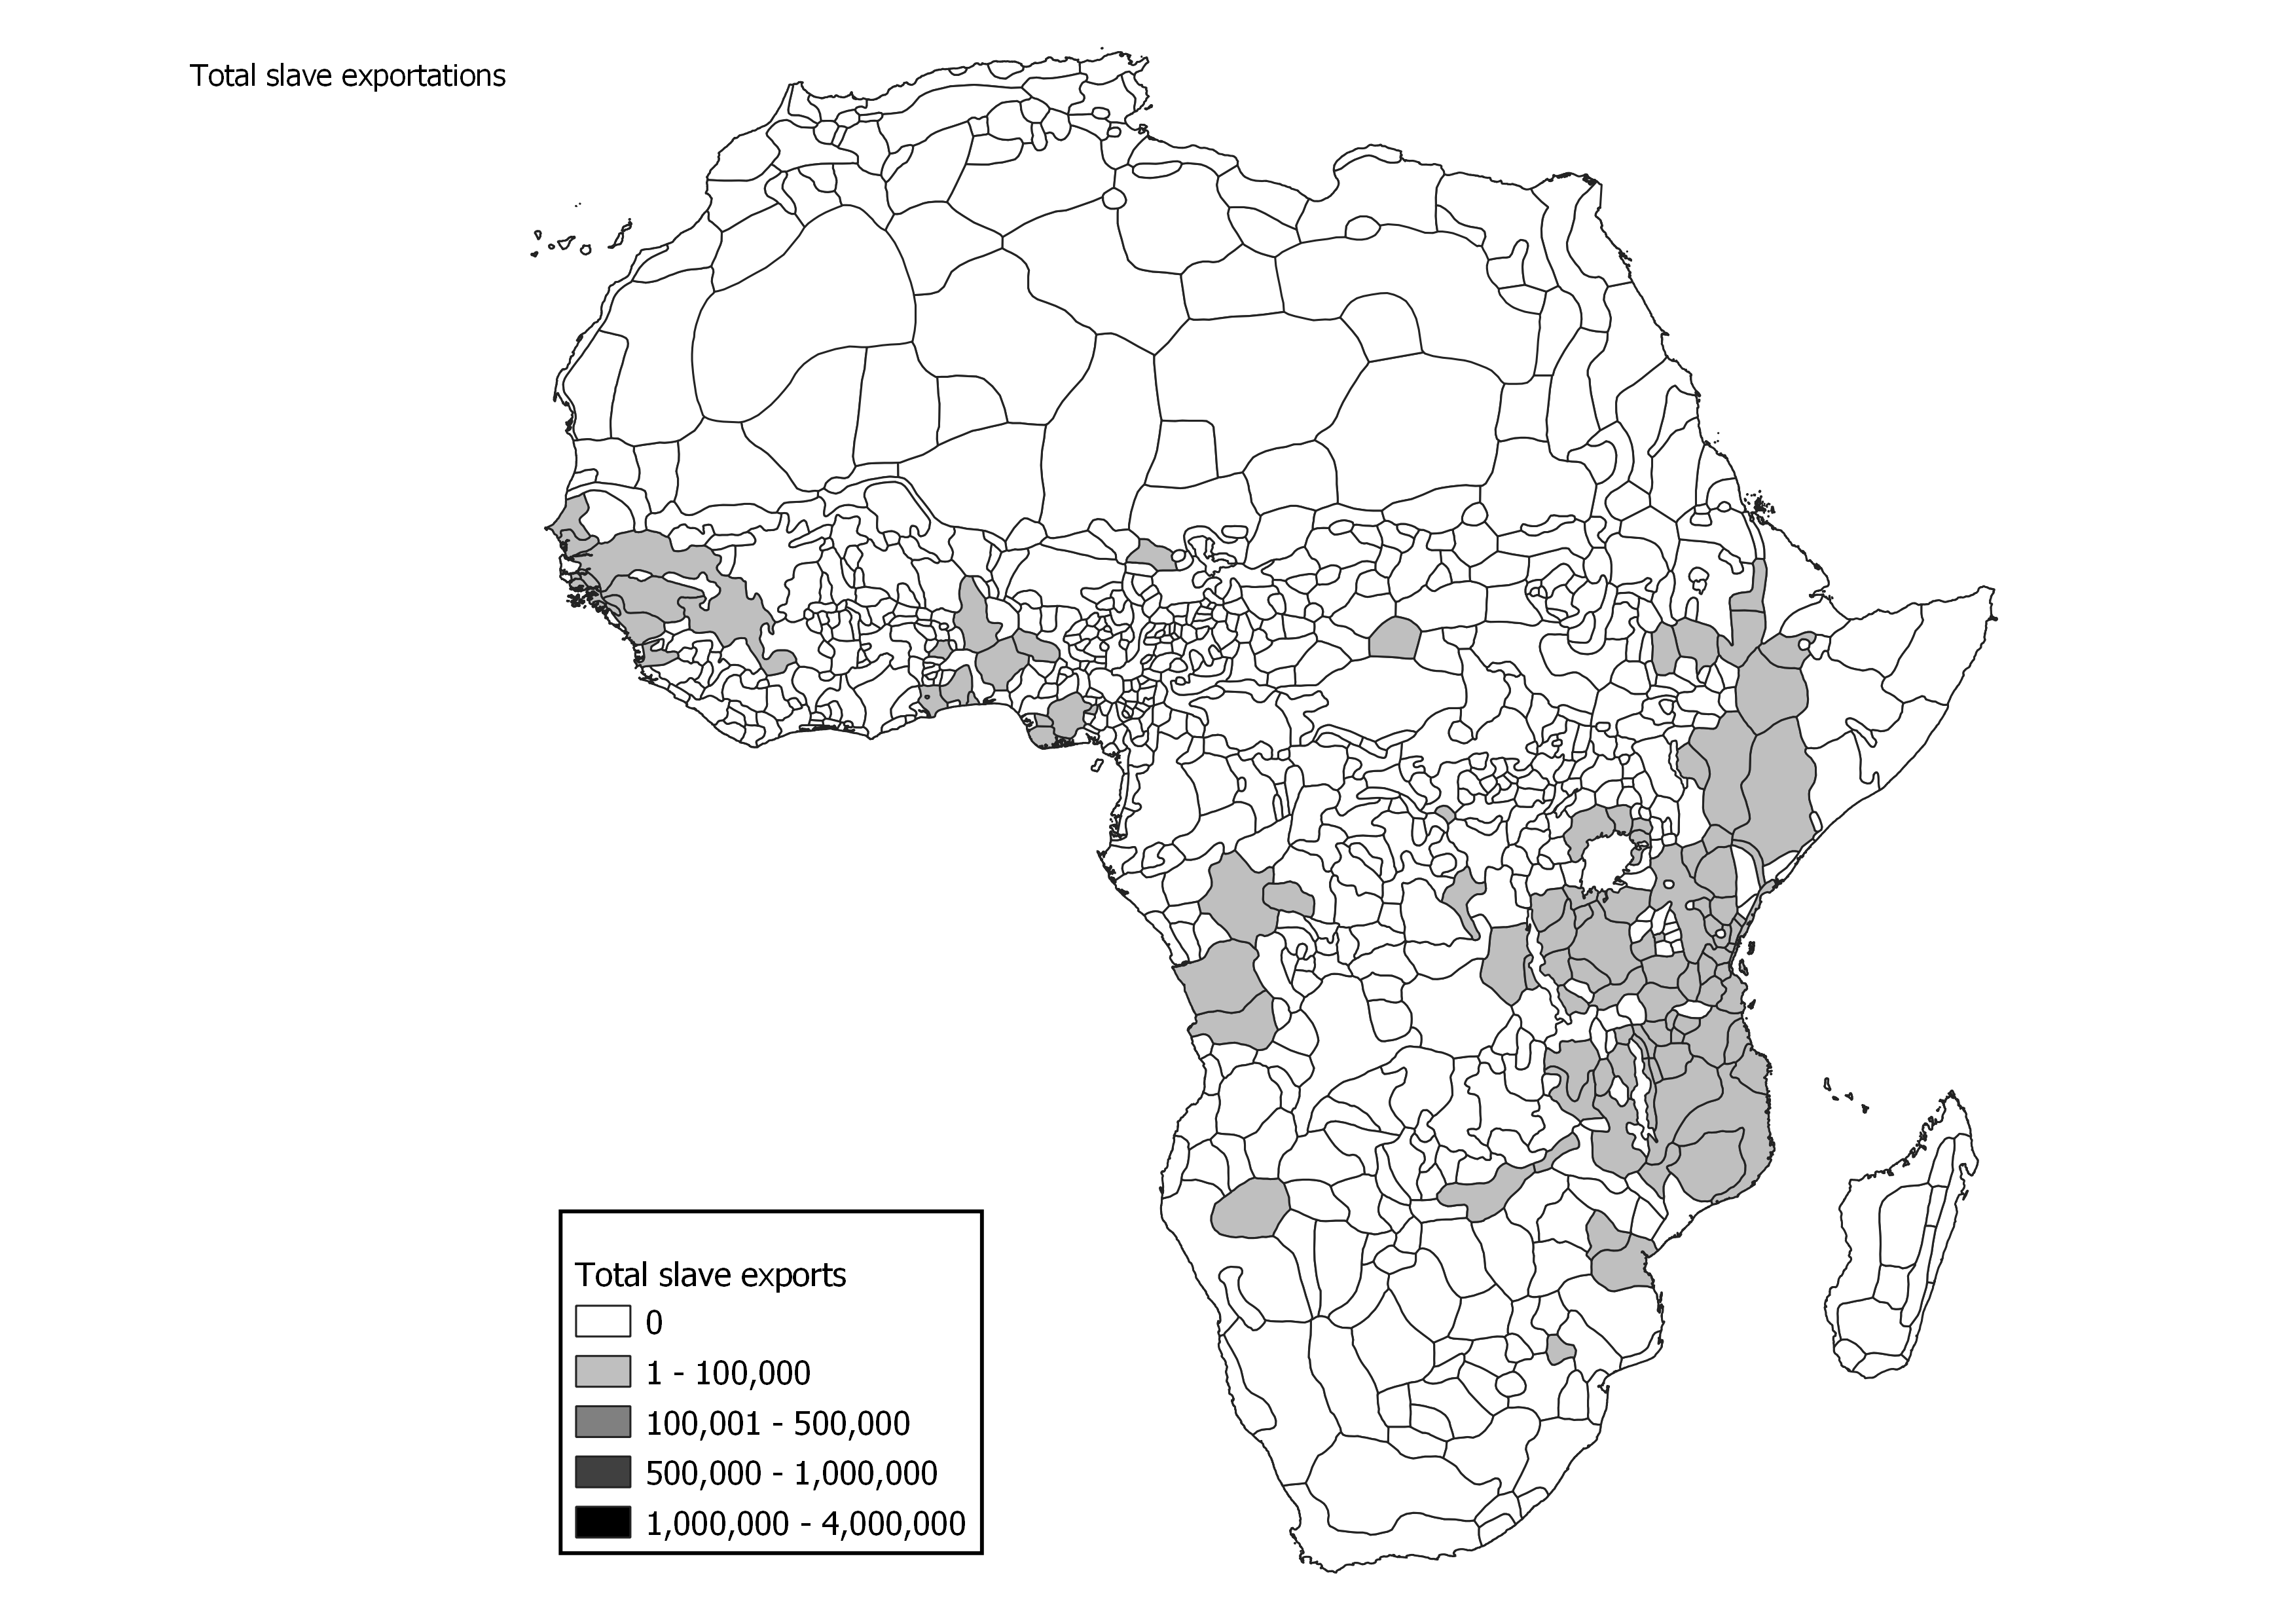
\includegraphics[scale = 0.45]{Final/totalslaveexports1500.png}
\label{}
\centering

Source: Own elaboration based on data sets of Nunn, N., \& Wantchekon, L. (2011): The slave trade and the origins of mistrust in Africa. American Economic Review.
\end{figure}

\begin{figure}[H]
\caption{}
\centering
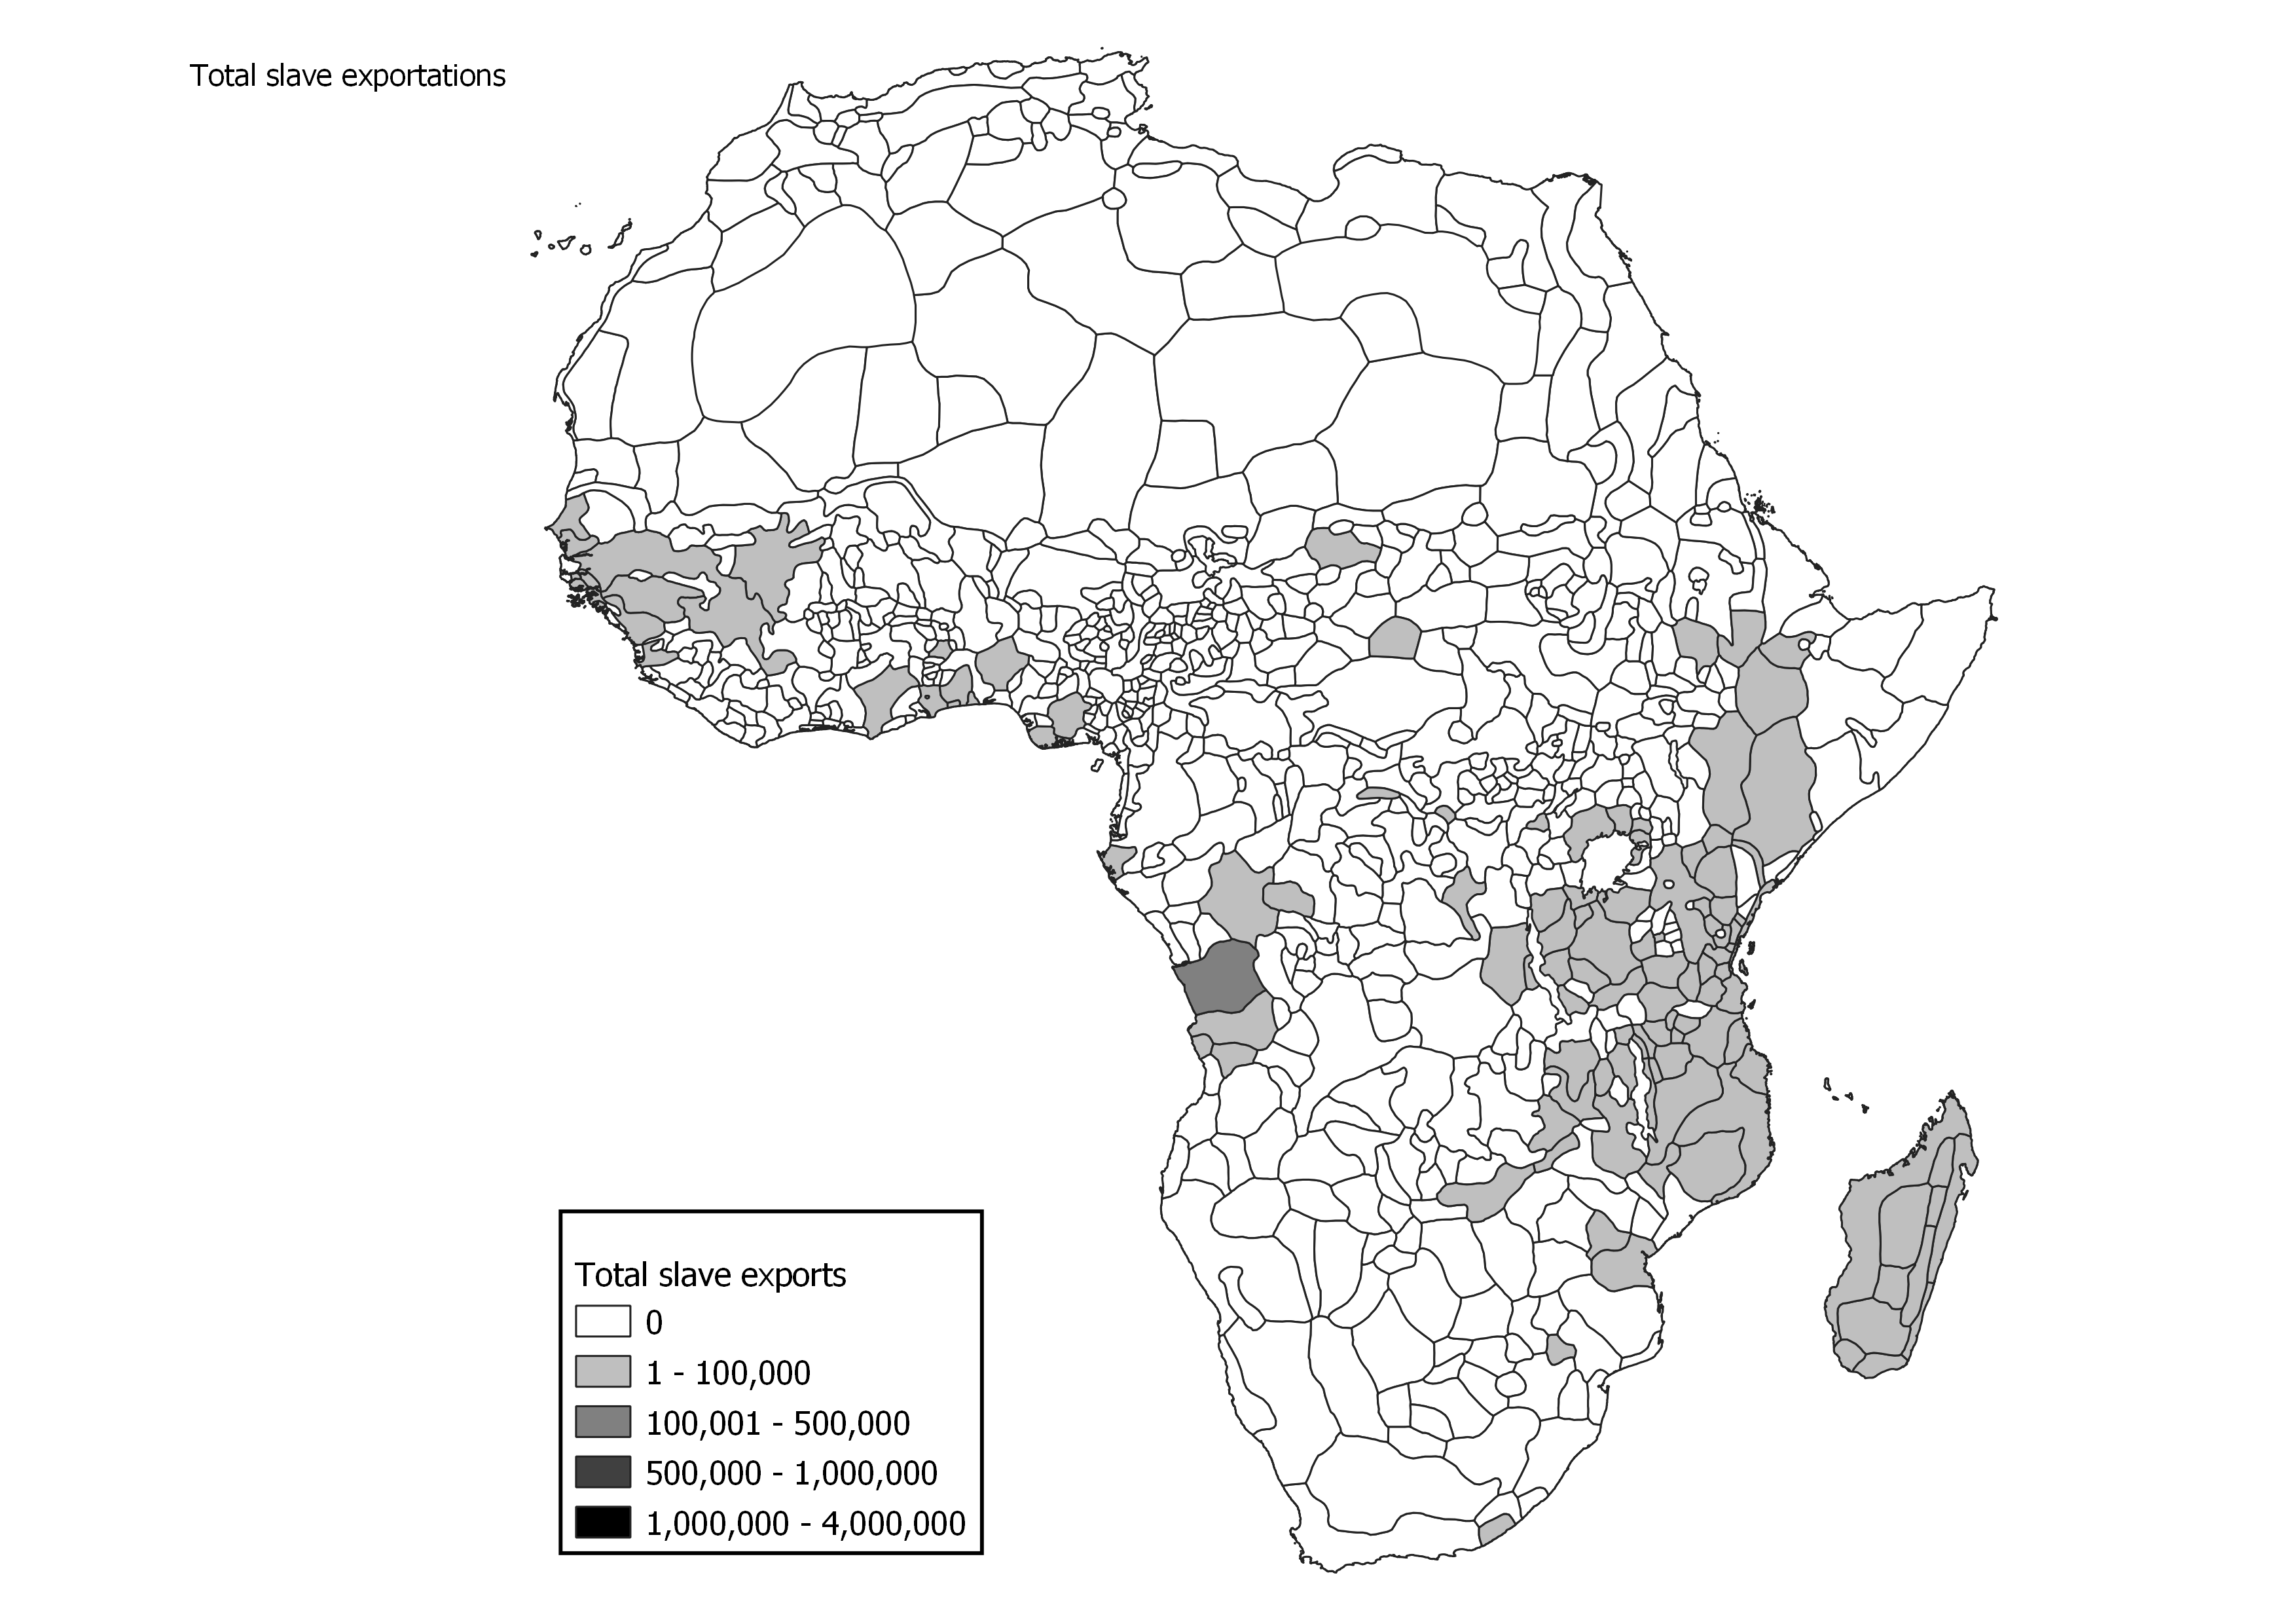
\includegraphics[scale = 0.45]{Final/totalslaveexports1600.png}
\label{}
\centering

Source: Own elaboration based on data sets of Nunn, N., \& Wantchekon, L. (2011): The slave trade and the origins of mistrust in Africa. American Economic Review.
\end{figure}

\begin{figure}[H]
\caption{}
\centering
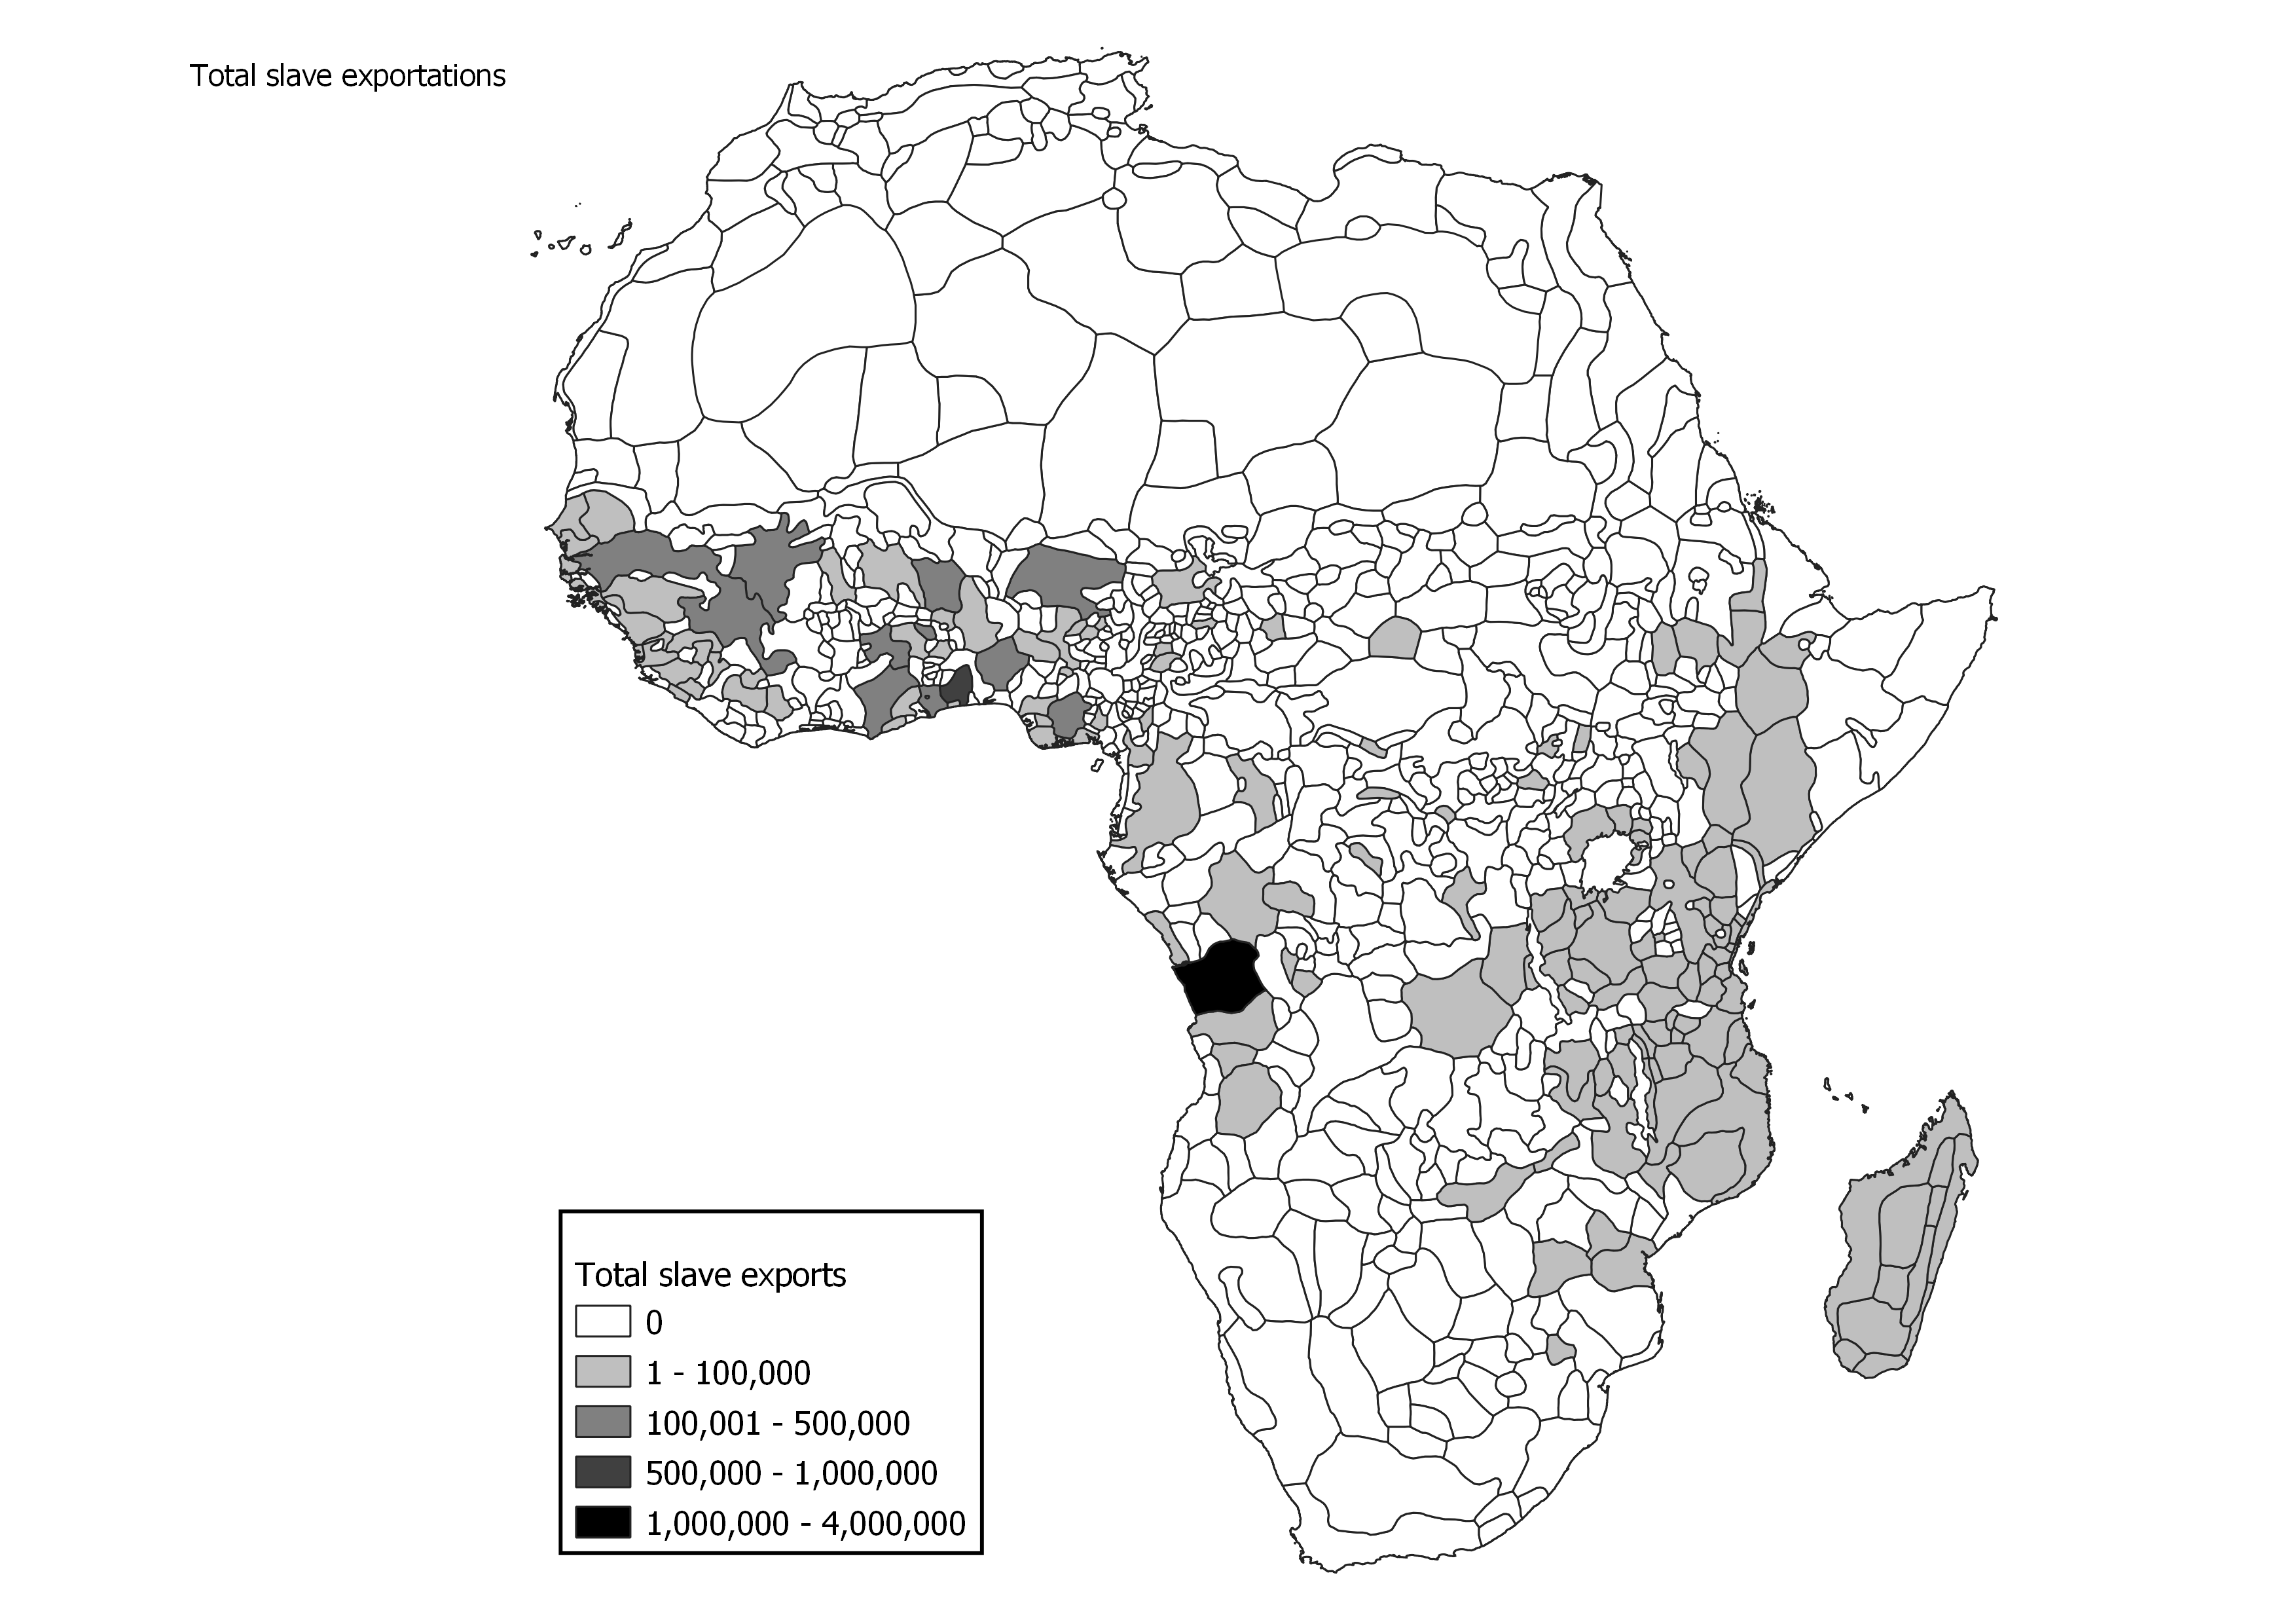
\includegraphics[scale = 0.45]{Final/totalslaveexports1700.png}
\label{}
\centering

Source: Own elaboration based on data sets of Nunn, N., \& Wantchekon, L. (2011): The slave trade and the origins of mistrust in Africa. American Economic Review.
\end{figure}

\begin{figure}[H]
\caption{}
\centering
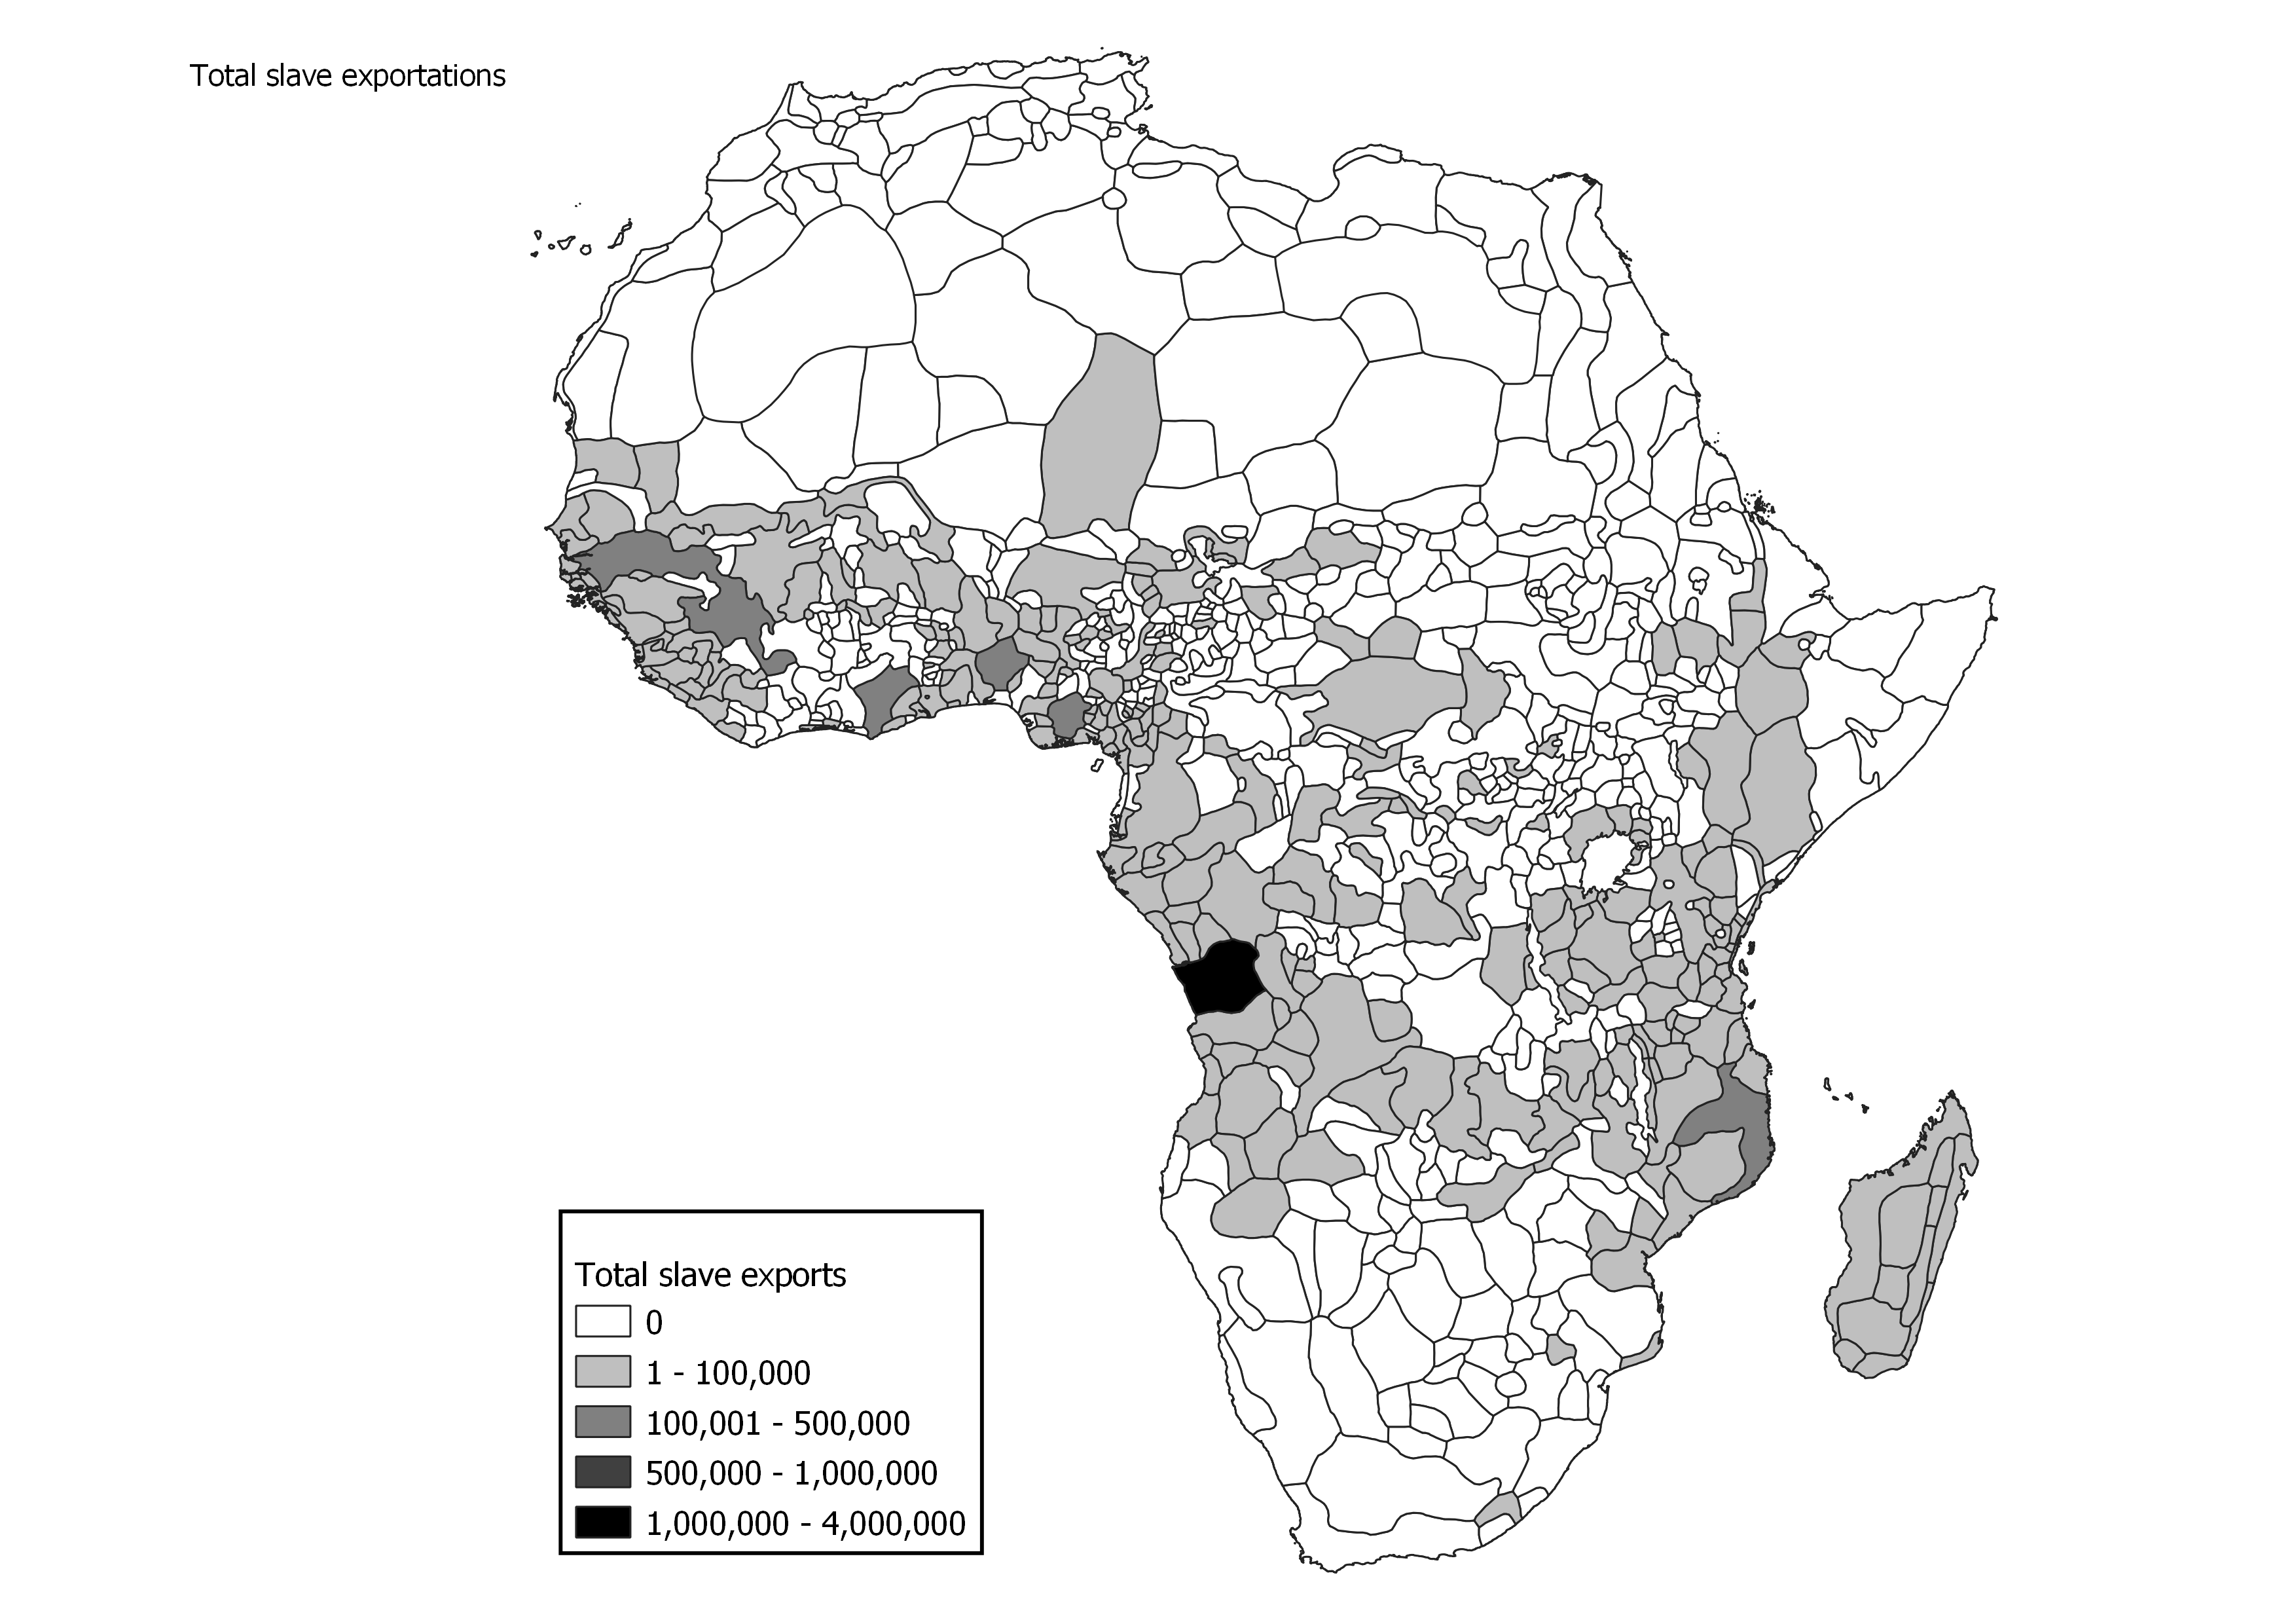
\includegraphics[scale = 0.45]{Final/totalslaveexports1800.png}
\label{}
\centering

Source: Own elaboration based on data sets of Nunn, N., \& Wantchekon, L. (2011): The slave trade and the origins of mistrust in Africa. American Economic Review.
\end{figure}

\end{document}
